\documentclass[A4paper,12pt]{report}



%******************************************************************* voici mes packages
\usepackage[utf8]{inputenc}  %les package responsable sur la langue
\usepackage[T1]{fontenc}
\usepackage[french]{babel}
%\usepackage{ae}
\usepackage{amsmath}   %les packages responsable sur la gestion des écriture mathématiques
\usepackage{amsfonts}
\usepackage{amssymb}
\usepackage{amsthm}
\usepackage{amscd}
%\usepackage{bbold}
\usepackage{amstext}
\usepackage{mathrsfs}
\usepackage{hyperref}
\usepackage[left=2.30cm, right=2.30cm, top=2.00cm, bottom=2.00cm]{geometry}
\usepackage{graphicx}% la gestion des images et les cadres
\usepackage{fancybox} %la gestion des cadres
\usepackage{xcolor}%la gestion des couleur

\usepackage{stmaryrd}%la gestion des crochets doublés...
\usepackage{textcomp}
\usepackage{graphicx}
\usepackage{indentfirst}% pour l'indentations des paragraphes

\def\Perp{\perp\!\!\!\perp}

%\definecolor{dodo}{rgb}{0.4,0.8,0.4}
\definecolor{red1}{rgb}{0.9,0.5,0.4}
\colorlet{red2}{red!70!black}
\definecolor{red3}{rgb}{0.9,0.2,0.2}
\usepackage{bookmark} %pour la gestion des reference dans mon pdf
%\usepackage{hyperref}
\hypersetup{
colorlinks=true,
linkcolor= red2,
urlcolor=red1
}



%\usepackage{tocloft}
%\renewcommand{\cftdot}{*}


\usepackage{multirow}% la gestion de tableau, fusionnement
\usepackage{multicol}

\usepackage{fancybox}

\usepackage{sectsty}
\sectionfont{\color{blue}}
\subsectionfont{\color{red3}}

\usepackage{fancyhdr}
\pagestyle{fancy}
\fancyhf{}
%\lhead{\thesechapter}
%\renewcommand{\headrulewidth}{0.5pt}
%\fancyhead[C]{ \rightmark} 
\fancyhead[L]{\rightmark}
\fancyhead[R]{}

\renewcommand{\footrulewidth}{0.5pt}
\fancyfoot[L]{ } % c'est a dire afficher le nombre de la page dans le centre du pied de la page
%\fancyfoot[L]{{\tiny Faculté des sciences Oujda, Labo ACSA}} % afficher 'chems-eddin' dans le pied de la page a gauche
%\fancyfoot[L]{{\tiny Faculté des sciences Oujda, Labo ACSA}}
\fancyfoot[C]{\textbf{page }\thepage}  % afficher 'atelier 4' dans le pied de la page a droit


%********************************************************************************************
\newtheorem{acknowledgement}{Acknowledgement}[section]
 
 
\newtheorem{proposition}{Proposition}[chapter]
\newtheorem{theorem}{Th\'eor\`eme}[chapter]
\newtheorem{exercice}{Exercice}[chapter]
\newtheorem{definition}{D\'efinition}[chapter]
\newtheorem{remark}{Remarque}[chapter]
\newtheorem{example}{Exemple}[chapter]
\newtheorem{corollary}{Corollaire}[chapter]
\newtheorem{lemma}{Lemme}[chapter]
\newtheorem{notation}{Notation}[chapter]

\usepackage[Conny]{fncychap}

\usepackage{enumerate}
\usepackage{float}
\usepackage{makeidx}
\makeindex	
%\title{Introduction à la Théorie algébrique des nombres}
%\author{M.C. ISMAILI\footnote{mcismaili@yahoo.fr} et M.M. CHEMS-EDDIN\footnote{2m.chemseddin@gmail.com}}

%\address{Mohamed Mahmoud CHEMS-EDDIN: Mohammed First University, Mathematics Department, Sciences Faculty, Oujda, Morocco }
%\email{2m.chemseddin@gmail.com}


	
%%%%%%%%%%%%%%%%%%%%%%%%%%%%%%%%%%%%%%%%%%%%%%%%%%%%%%%%%%%%%%%%%%%%
%%%%%%%%%%%%%%%%%%%%%%%%%%%%%%%%%%%%%%%%%%%%%%%%%%%%%%%%%%%%%%%%chp1
%	\newtheorem{thm}{\bf Th\'eor\`eme}[chapter]
	\newtheorem{dfn}{ D\'efinition}[chapter]
	\newtheorem{cor}{ Corollaire}[chapter]
	\newtheorem{ex}{ Exemple}[chapter]
	\newtheorem{lem}{ Lemme}[chapter]
	\newtheorem{exs}[ex]{ Exemples}
	\newtheorem{con}{Conjecture}[chapter]
%	\newtheorem{prop}{ Proposition}[chapter]
	\newtheorem{propr}{ Propriété}[chapter]
	\newtheorem{prob}{ Probl\`{e}me}[chapter]
	\newtheorem{rem}{ Remarque}[chapter]
	\newtheorem{rems}[rem]{ Remarques}
	\newtheorem{nota}{ Notation}[chapter]
	\newtheorem{notas}[nota]{Notations}
		\newtheorem{exo}{Exercice}[chapter]
	
	
	\thispagestyle{empty}  \baselineskip 6mm
	\newcommand{\Kro}{{\em Kronecker\/}}
	\newcommand{\Web}{{\em Weber\/}}
	\newcommand{\Hil}{{\em Hilbert\/}}
	\newcommand{\Tak}{{\em Takagi\/}}
	\newcommand{\Fur}{{\em Furtw\"{a}ngler\/}}
	\newcommand{\Art}{{\em Artin\/}}
	\newcommand{\Fer}{{\em Fermat\/}}
	\newcommand{\Has}{{\em Hasse\/}}
	\newcommand{\Eul}{{\em Euler\/}}
	\newcommand{\Dir}{{\em Dirichlet\/}}
	\newcommand{\Ded}{{\em Dedekind\/}}
	%\newcommand{\Gau}{{\em Gauss\/}}\
	
	\newcommand{\Kum}{{\em Kummer\/}}
	\newcommand{\kro}{Kronecker}
	\newcommand{\ded}{Dedekind}
	\newcommand{\dir}{Dirichlet}
	\newcommand{\ka}{{\bf k}}
	\newcommand{\K}{{\bf K}}
	\newcommand{\R}{{\mathbb{R}}}
	\newcommand{\Ll}{{\bf L}}
	\newcommand{\Q}{{\mathbb{Q}}}
	\newcommand{\N}{{\mathbb{N}}}
	\newcommand{\C}{{\mathbb{C}}}
	\newcommand{\Z}{{\mathbb{Z}}}
	\newcommand{\E}{{\mathbb{E}}}
	\newcommand{\pr}{{\mathbb{P}}}
	\newcommand{\Hb}{{\bf H}}
	\newcommand{\Hh}{{\bf H}}
	\newcommand{\Kk}{{\bf K/k}}
	\newcommand{\kkk}{{\bf K/k}}
	\newcommand{\rmt}{\mbox{$\sqrt{-m}$}}
	\newcommand{\ra}[1]{\mbox{$\sqrt{#1}$}}
	\newcommand{\zs}{\mbox{$\zeta(s)$}}
	\newcommand{\jo}{\mbox{$j(\omega)$}}
	%\newcommand{\mod}[3]{\mbox{${#1} \equiv{#2}\bmod{#3}$}}
	\newcommand{\icg}{ideal class group}
	\newcommand{\cf}{class field}
	\newcommand{\cft}{class field theory}
	\newcommand{\kcf}{Kronecker class field}
	\newcommand{\hcf}{Hilbert class field}
	\newcommand{\acf}{absolute class field}
	\newcommand{\ext}{extension}
	\newcommand{\cmp}{complex multiplication}
	\newcommand{\m}{\mbox{$\cal M$}}
	\newcommand{\p}{\mbox{$\cal P$}}
	\newcommand{\am}{\mbox{$A_{\cal M}$}}
	\newcommand{\hm}{\mbox{$H_{\cal M}$}}
	\newcommand{\ag}{\mbox{$\cal A$}}
	\newcommand{\xg}{\mbox{$\cal X$}}
	\newcommand{\cm}{\mbox{$C_{\cal M}$}}
	\newcommand{\lsxk}{\mbox{$L(s,\chi,{\bf k})$}}
	\newcommand{\ogo}{\mbox{$\cal O$}}
	\newcommand{\lims}{\mbox{$$\lim_{s \rightarrow 1+}$$}}
	\newcommand{\of}{\mbox{${\bf o}_{f}$}}
	\newcommand{\ok}{\mbox{${\bf o}_{\bf k}$}}
	\newcommand{\gam}{\mbox{${\bf \Gamma}$}}
	\newcommand{\sm}{\mbox{$\sigma$}}
	\newcommand{\cH}{\cal H}
	\newcommand{\cM}{\cal M}
		%\renewcommand{\mathcal{P}}{\mathcal{P}}
%%%%%%%%%%%%%%%%%%%%%%%%%%%%%%%%%%%%%%%%%%%%%%%%%%%%%%%%%%%%%%%%%%%%
%%%%%%%%%%%%%%%%%%%%%%%%%%%%%%%%%%%%%%%%%%%%%%%%%%%%%%%%%%%%%%%%chp2	

	
	
	
	
	
	
	
	

\begin{document}
\begin{titlepage}
   
   
%\begin{figure}[h!]
 %   \centering
  %  \includegraphics[scale = 1]{fsdm.png}
%\end{figure}


\begin{center}
    
\includegraphics[width=0.3\textwidth]{logo}\par\vspace{1cm}
\end{center}

\thispagestyle{empty}
\centering  
\vspace{0.6cm}
\textsf{\textbf{\large Mémoire présenté à \\La Faculté des Sciences Dhar El Mahraz Fès}}\\\vspace{0.3cm}
\textsf{\textbf{\LARGE Master Mathématiques \\ Appliquées et Science des Données (MASD)}}\\	\vspace{0.5cm}
%\textsf{\textbf{\large Master en double diplomation avec l’Université Sorbonne Paris Nord}}\\\vspace{0.5cm}
\textsf{\textbf{\large Spécialité : Statistique et Science des Données}}\\	\vspace{0.5cm}
\textsf{\textbf{\large Intitulé :}}\vspace{0.2cm}
\noindent\makebox[\linewidth]{\rule{\linewidth}{1.2pt}}	
 \textcolor{blue!80!black}{\\\LARGE \LARGE \LARGE\LARGE \textsf{ \textbf{  Étude de stabilité des équations différentielles stochastiques}}}
\noindent\makebox[\linewidth]{\rule{\linewidth}{1.2pt}}
% my name prenom
\vspace{0.12cm}
   \textsf{\large \\\textbf{Présenté par: OUMARGHAD Abdelaziz}}\\\vspace{0.13cm}
   \textsf{\large \textbf{Encadré par: EL BARRIMI Oussama}}\\\vspace{0.13cm}
   %\textsf{\large \textbf{Co-encadré par: }}\\
   	\vspace{1.5cm}
	\smallskip
	\large \fontfamily{ptm}\fontseries{m}\selectfont{ \textsf{Soutenu le 19/06/2023, devant le jury }}  \\
	\vspace{0.5cm}
\begin{minipage}{0.4\textwidth}
    \begin{flushleft}
     \textsf{\textbf{Pr.} KIOUACH Driss}\\
     \textsf{\textbf{Pr.} BARBARA Abdelkrim}\\
     \textsf{\textbf{Pr.} EL BARRIMI Oussama}\\
    \end{flushleft}
\end{minipage}
\begin{minipage}{0.2\textwidth}
    \begin{flushleft}
    \textsf{ président}\\
    \textsf{ Examinateur}\\
    \textsf{ Encadrant}\\
    \end{flushleft}
\end{minipage}
\begin{minipage}{0.3\textwidth}
    \begin{flushleft}
      \textsf{Etablissement \textbf{ FSDM}}\\
      \textsf{Etablissement \textbf{ FSDM}}\\
      \textsf{Etablissement \textbf{ FSDM}}\\
    \end{flushleft}
\end{minipage}
	\vspace{2cm}
%\begin{picture}(150,44)
\begin{center}
\textcolor{blue!80!black}{\textbf{\textsf{ \large Ann\'ee Universitaire : 2022-2023}}}
\end{center}
%\end{picture}
\end{titlepage}


\chapter*{Remerciement}
Je tiens à exprimer mes chaleureuses remerciements au professeur \textbf{\textit{EL BARRIMI Oussama}}, pour sa grande disponibilité, ses conseils avisés et pour l'aide qu'il m'a apporté dans rédaction et la conception de ce mémoire.   

Je tiens également à exprimer ma profonde gratitude envers les membres du jury professeur \textbf{\textit{BARBARA Abdelkrim}}, et professeur \textbf{\textit{KIOUACH Driss}},  qui ont accepté de consacrer leur temps et leur expertise pour évaluer ce travail, d'apporter des commentaires constructifs, des observations perspicaces et des suggestions  extrêmement précieuses pour enrichir ce travail.

Mes plus vifs remerciements vont aussi envers toute l’équipe pédagogique du master MASD qui a rendu possible ce projet  et qui a soutenu mes efforts tout au long de ce parcours.


	
	
	
	
	
\chapter*{Introduction}	
Les équations différentielles sont un outil fondamental pour modéliser des phénomènes dynamiques. Elles permettent de décrire l'évolution d'une quantité en fonction de ses dérivées et de variables indépendantes. Traditionnellement, les équations différentielles déterministes ont été utilisées pour modéliser des systèmes où toutes les variables sont parfaitement prévisibles. Cependant, dans de nombreux domaines, notamment en finance, en physique et en biologie, il est fréquent de rencontrer des phénomènes caractérisés par une certaine dose de bruit ce qui a imposé le développement d'un cadre plus particulier qui traite ce bruit et qui fourni un cadre mathématique puissant pour modéliser les systèmes dynamiques sous l'influence de facteurs imprévisibles ou incertains qui peuvent provenir de fluctuations aléatoires, de perturbations externes ou de l'interaction complexe entre les composantes d'un système. Ce développement remonte au début du XXe siècle, lorsque les mathématiciens ont commencé à explorer la modélisation des phénomènes dynamiques sous l'influence de l'incertitude. Plusieurs contributeurs majeurs ont contribué à l'évolution de ce domaine, en développant des concepts clés et des méthodes pour aborder les systèmes dynamiques stochastiques.

L'un des pionniers importants de l'étude des équations différentielles stochastiques est le mathématicien français Paul Lévy. Dans les années 1930, Lévy a jeté les bases de la théorie des processus stochastiques, ses travaux ont permis d'introduire des notions fondamentales, telles que les intégrales stochastiques, ensuite, dans les années 1940, le mathématicien japonais Kiyosi Itô, a formulé le célèbre calcul stochastique, également connu sous le nom de calcul d'Itô. Ce calcul fournit des outils mathématiques rigoureux pour manipuler les processus stochastiques et résoudre les équations différentielles stochastiques. Le calcul d'Itô a ouvert de nouvelles perspectives en permettant l'analyse et la résolution de problèmes complexes impliquant des phénomènes aléatoires.

Au fur et à mesure que la théorie des processus stochastiques et le calcul stochastique se développaient, les équations différentielles stochastiques ont commencé à être appliquées dans divers disciplines scientifiques et techniques. Dans les années 1950 et 1960, les mathématiciens ont exploré l'application des équations différentielles stochastiques à la finance, en particulier à la modélisation des marchés financiers et des prix d'actifs.

Dans les décennies suivantes, l'étude des équations différentielles stochastiques s'est étendue à de nombreux autres domaines, tels que la physique, la biologie, l'économie et  la chimie. Des chercheurs du monde entier ont apporté d'importantes contributions à ce domaine, en développant de nouvelles méthodes numériques pour résoudre les équations différentielles stochastiques et en explorant des applications spécifiques à chaque domaine.

De nos jours, les équations différentielles stochastiques occupent une place centrale dans la modélisation et l'analyse des systèmes dynamiques complexes, où l'incertitude et les fluctuations aléatoires jouent un rôle essentiel. L'étude de ces équations continue d'évoluer, avec de nouvelles avancées théoriques et des applications innovantes dans divers domaines de la science, de la technologie et de la finance.

Dans ce mémoire, nous commencerons par rappeler certaines notions du calcul stochastique telles que les processus à temps continu, le mouvement Brownien et les fondements de l'intégration stochastique. Dans le deuxième chapitre, nous aborderons les équations différentielles stochastiques, discuter l'existence et l'unicité des solutions. Dans le troisième chapitre, nous examinerons la variation des solutions par rapport aux conditions initiales, en supposant l'unicité des trajectoires.
\tableofcontents	

\chapter{Éléments du calcul stochastique}
\section{Processus stochastiques}
\subsection{Notions fondamentales}
On se donne $(\Omega, \mathcal{F}, \pr)$ un espace de probabilité complet i.e. si $B \in \mathcal{F}$ tel que $\pr(B)=0$ et $A \subset B$, alors $A \in \mathcal{F}$

Une base stochastique est la donnée de $\left(\Omega, \mathcal{F},\left(\mathcal{F}_{t}\right)_{t \geq 0}, \pr \right)$ où $\left\{\mathcal{F}_{t}, t \geq 0\right\}$ est une famille de sous tribus de $\mathcal{F}$ telle que $\mathcal{F}_{s} \subset \mathcal{F}_{t}$ pour tout $s \leq t .\left\{\mathcal{F}_{t}, t \geq 0\right\}$ s'appelle une filtration.

Hypothèses (conditions) habituelles: On dit que $\left(\Omega, \mathcal{F},\left(\mathcal{F}_{t}\right)_{t \geq 0}, \pr \right)$ satisfait les conditions habituelles si : $\mathcal{F}_{0}$ contient tous les $P$-négligeables et $\mathcal{F}_{t}$ est continue à droite i.e. $\mathcal{F}_{t}=\cap_{s>t} \mathcal{F}_{s}$.
 \begin{definition}
 Un processus stochastique $X:=\left\{X_{t}, t \geq 0\right\}$ est une collection de v.a. $X_{t}, t \geq 0$ :

$$
\begin{aligned}
X_{t}: \quad \Omega & \longrightarrow \mathbb{R}^{n} \\
\omega &\longrightarrow X_{t}(\omega) .
\end{aligned}
$$

On dira que le processus $\left\{X_{t}, t \geq 0\right\}$ est adapté à $\mathcal{F}_{t}$ si $\forall t \geq 0 X_{t}$ est $\mathcal{F}_{t}$-mesurable. L'application (pour $\omega \in \Omega$ fixé)

$$
\begin{aligned}
 X .(\omega): \quad \mathbb{R}_{+} &\longrightarrow \mathbb{R}^{n} \\
 t & \longrightarrow X_{t}(\omega)
\end{aligned}
$$

s'appelle une trajectoire du processus.
\end{definition}
\begin{definition}
 Soient $X$ et $Y$ deux processus stochastiques, définis sur le même espace de probabilité. On dira que $X$ est une modification de $Y$ si

$$
\forall t \geq 0 \quad \pr \left[X_{t}=Y_{t}\right]=1 .
$$

i.e. $\forall t \geq 0$, il existe $\mathcal{N}_{t}$ négligeable tel que $\forall \omega \notin \mathcal{N}_{t}$ on ait $X_{t}(\omega)=Y_{t}(\omega)$
\end{definition}

\begin{remark} 
En général la notation $\mathcal{N}$ sera réservée aux ensemble négligeables
\end{remark}

\begin{definition}  Deux processus stochastiques $X$ et $Y$ sont dits indistingables si

$$
\pr \left[X_{t}=Y_{t} \quad \forall t \geq 0\right]=1 .
$$

i.e. Il existe $\mathcal{N}$ négligeable tel que $\forall \omega \notin \mathcal{N}$ et $\forall t \geq 0$, on a $X_{t}(\omega)=Y_{t}(\omega)$.
\end{definition}
\begin{definition}
Un processus stochastique $X$ est dit continu s'il existe $\mathcal{N}$ négligeable tel que $\forall \omega \notin \mathcal{N}$ l'application $t \mapsto X_{t}(\omega)$ soit continue.
\end{definition}
\subsection{Variation d'ordre p d'un processus}
\begin{definition}
Soient $X=(X_t, t\geq 0)$ un processus stochastique, $T>0$, $\sigma=\left(t_{i}\right)_{0 \leq i \leq n}$ une subdivision  de $[0, T]$ (i.e) une suite de nombres t.q. $0=t_{0} \leq t_{1} \cdots \leq t_{n}=T$

On définit la variation infinitésimale d'ordre $p$ du processus $X$ sur $[0, T]$ associée à la subdivision $\sigma$ de $[0, T]$ par :
$$
V_{T}^{p}(X, \sigma):=\sum_{i=1}^{n}\left|X_{t_{i}}-X_{t_{i-1}}\right|^{p} 
$$
\end{definition}

Si $V_{T}^{p}(X, \sigma)$ a une limite lorsque $\|\sigma\|_{\infty}:=\sup _{1 \leq i \leq n-1}\left|t_{i+1}-t_{i}\right| \rightarrow 0$, la limite ne dépend pas de la subdivision choisie et nous l'appellerons variation d'ordre $p$ de $X$ sur $[0, T]$.

En particulier:
\begin{enumerate}
\item si $p=1$, la limite s'appellera variation totale de $X$ sur $[0, T]$.

\item si $p=2$, la limite s'appellera variation quadratique de $X$ sur $[0, T]$ notée $\langle X\rangle_{t}$.
\end{enumerate}

De plus on dit que $X$ est:
\begin{itemize}
\item à variation bornée sur $[0,T]$ si $\exists K>0$ tel que: $$\sup \sum_{i=0}^{n-1} \lvert X_{t_{i+1}} - X_{t_i} \rvert \leq K $$
\item à variation finie sur $[0,T]$ si: $$\sup \sum_{i=0}^{n-1} \lvert X_{t_{i+1}} - X_{t_i} \rvert < + \infty$$
\end{itemize}
le supremum étant pris sur les subdivisions $\sigma=\left(t_{i}\right)_{0 \leq i \leq n}$. 
\subsection{Martingales, sous-martingales et sur-martingales}

\begin{definition} 
 Soit $M=\left\{M_{t}, t \geq 0\right\}$ un processus stochastique dans $L^{1}(\Omega, \mathcal{F}, \pr )$ i.e. $\forall t \geq 0, E\left|M_{t}\right|<$ $+\infty$ adapté à la filtration $\left\{\mathcal{F}_{t}, t \geq 0\right\}$
\begin{enumerate}
\item $M$ est dite martingale si: $$\forall  s<t, E\left[M_{t} / \mathcal{F}_{s}\right]=M_{s}$$

\item $M$ est dite sousmartingale si:  $$ \forall s<t, E\left[M_{t} / \mathcal{F}_{s}\right] \geq M_{s}$$

\item $M$ est dite surmartingale si: $$ \forall s<t, E\left[M_{t} / \mathcal{F}_{s}\right] \leq M_{s}$$
\end{enumerate}

\end{definition} 
\begin{propr}
\begin{enumerate}
     \item Si $M$ est une martingale $E\left[M_{t}\right]=E\left[M_{0}\right]$, pour tout $t$.

     \item Si $\left\{M_{t}, 0 \leq t \leq T\right\}$ est une martingale, le processus est complètement déterminé par sa valeur terminale : $M_{t}=E\left[M_{T} / \mathcal{F}_{t}\right]$.
\end{enumerate}
\end{propr}
Cette dernière propriété est d'un usage très fréquent en finance mathématique.

\begin{example}
 Soit $Y$ une v.a. intégrable. On pose $M_{t}=E\left[Y / \mathcal{F}_{t}\right],\left\{M_{t}, t \geq 0\right\}$ est une $\mathcal{F}_{t}$-martingale.

En effet: $M$ est $\mathcal{F}_{t}$-adapté par définition de l'espérance conditionnelle.

$E\left|M_{t}\right|=E\left|E\left[Y / \mathcal{F}_{t}\right]\right| \leq E\left[E\left[|Y| / \mathcal{F}_{t}\right]\right]=E|Y|<+\infty$

Soit $s<t, E\left[M_{t} / \mathcal{F}_{s}\right]=E\left[E\left[Y / \mathcal{F}_{t}\right] / \mathcal{F}_{s}\right]=E\left[Y / \mathcal{F}_{s}\right]=M_{s}$.\\
\end{example}
\begin{example}
 Soient $\phi$ une fonction convexe, croissante, $\left(M_{t}, \mathcal{F}_{t}\right)$ est une sousmartingale telle que $\phi\left(M_{t}\right)$ soit intégrable pour tout $t \geq 0$. Alors $\left(\phi\left(M_{t}\right), \mathcal{F}_{t}\right)$ est une sousmartingale.
\end{example}
\subsection{Temps d'arrêt}
\begin{definition} 
(Temps d'arrêt) Soit $T: \Omega \rightarrow \overline{\mathbb{R}}_{+}$une v.a. T est dit un temps d'arrêt si $\{T \leq t\} \in \mathcal{F}_{t}$ quel que soit $t \geq 0,\{T \leq t\}=\{\omega \in \Omega: T(\omega) \leq t\}$. 
\end{definition} 
\begin{theorem} Si $S$ et $T$ sont deux temps d'arrêt alors $S \vee T, S \wedge T, \alpha S$, pour $\alpha>1$ et $S+T$ sont des temps d'arrêt.
\end{theorem}
Ce résultat peut s'étendre à tous les temps d'arrêt si on impose à notre martingale d'être  uniformément intégrable.
Définissons d'abord les notions d'intégrabilité uniforme, et de la tribu des événements antérieurs.
\begin{definition} Une famille de v.a. $\left\{X_{t}, t \in [0, T]\right\}$ est dite uniformément intégrable si

$$
\lim _{C \rightarrow+\infty} \sup _{t \in [0, T]} \int_{\left\{\left|X_{t}\right| > C\right\}}\left|X_{t}\right| \mathrm{d} P=0,
$$
\end{definition}
\begin{definition}
 On associe à un temps d'arrêt $\tau$ la tribu $\mathcal{F}_{\tau}$ dite des événements antérieurs à $\tau$, définie par

$$
\mathcal{F}_{\tau}=\left\{A \in \mathcal{F}: A \cap \mathbf{1}_{\{\tau \leq t\}} \in \mathcal{F}_{t} \forall t \geq 0\right\} 
$$
\end{definition}
\begin{theorem}
Si $M$ est uniformément intégrable on a:
\begin{enumerate}
\item $M$ converge p.s. et dans $L^{1}$ vers $M_{\infty}$ quand $t \rightarrow+\infty$ 
\item pour tout temps d'arrêt $\tau$ nous avons $M_{\tau}=E\left[M_{\infty} / \mathcal{F}_{\tau}\right]$
\end{enumerate} 
\end{theorem}
\begin{proposition} Si pour tout temps d'arrêt borné $\tau, E\left[X_{\tau}\right]=E\left[X_{0}\right]$, le processus $X$ est une martingale.
\end{proposition}

\begin{proposition}
Si $S$ et $T$ sont des temps d'arrêt tels que $S \leq T$, alors $\mathcal{F}_{S} \subset \mathcal{F}_{T}$.
\end{proposition}
\begin{proposition}
Soit $\left\{X_{t}, t \geq 0\right\}$ un processus et $T$ un temps d'arrêt fini. On définit $X_{T}$ par $X_{T}(\omega)=X_{T(\omega)}(\omega)$ Si un processus $X$ est continu et adapté, $X_{\tau}$ est $\mathcal{F}_{\tau}$-mesurable.
\end{proposition}
\begin{proposition}
Si $T$ est un temps d'arrêt et soit $X=\left\{X_{t}, t \geq 0\right\}$ un processus continu, on note $X^{T}$ le processus arrêté $X_{t}^{T}=X_{t \wedge T}$ pour tout $t \geq 0$
\end{proposition}

\begin{definition} Un processus adapté à trajectoires continues $M=\left\{M_{t}, t \geq 0\right\}$ tel que $M_{0}=0$ p.s. est une martingale locale continue s'il existe une suite croissante de temps d'arrêt $\left\{T_{n}, n \in \mathbb{N}\right\}$ telle que $T_{n}$ croit p.s. vers $+\infty$ et pour tout $n$ le processus arrêté $M^{T_{n}}$ est une martingale uniformément intégrable.
\end{definition}

\begin{propr}
\begin{itemize}
\item[i)] Une martingale à trajectoires continues est une martingale locale $\left(T_{n}=n\right)$.

\item[ii)] Si $M$ est une martingale locale alors pour tout temps d'arrêt $T, M^{T}$ est une martingale locale.

\item[iii)] L'espace des martingales locales est un espace vectoriel.
\end{itemize}
\end{propr}

\begin{theorem}
Soit $M$ une martingale locale continue nulle en zéro i.e. $M_{0}=0$. Alors si $M$ est un processus à variation finie, $M$ est indistingable de 0 i.e. $M_{t}=0$ pour tout $t$ $P$-p.s.
\end{theorem}
\subsubsection{Théorème d'arrêt}
Si $T$ est un temps d'arrêt et $M$ une $\mathcal{F}_{t}$-martingale, le processus $Z$ défini par $Z_{t}:=M_{T \wedge t}$ est une $\mathcal{F}_{t}$-martingale. En particulier, $E\left[M_{T \wedge t}\right]=E\left[M_{0}\right]$.

\begin{theorem}[Théorème d'arrêt de Doob]
 Si $M$ est une $\mathcal{F}_{t}$-martingale continue et si $S$ et $T$ sont deux temps d'arrêt tels que $S \leq T \leq K, K$ étant une constante finie, $M_{T}$ est intégrable et

$$
M_{S}=E\left[M_{T} / \mathcal{F}_{S}\right]
$$
\end{theorem}
Ce résultat s'étend à tous les temps d'arrêt si la martingale est uniformément intégrable.

Si $M$ est uniformément intégrable, on peut montrer que $M_{t}$ converge p.s. et dans $L^{1}$ vers $M_{+\infty}$ quand $t \rightarrow+\infty$ et que $M_{\tau}=E\left[M_{+\infty} / \mathcal{F}_{\tau}\right]$

\begin{proposition} Si pour tout temps d'arrêt borné $\tau, E\left[X_{\tau}\right]=E\left[X_{0}\right]$, le processus $X$ est une martingale.
\end{proposition}


\begin{remark}
Si $E\left[X_{t}\right]=E\left[X_{0}\right]$ pour tout $t$, le processus $X$ n'est pas nécessairement une martingale. Un contre exemple est $X_{t}=\int_{0}^{t} M_{u} d u$ où $M$ est une martingale d'espérance nulle.\\
\end{remark}
\begin{remark}
Si $M$ est une surmartingale positive et $\tau$ un temps d'arrêt, $E\left[M_{\tau}\right] \leq E\left[M_{0}\right]$ où on pose $M_{+\infty}=0$.\\
\end{remark}
\begin{remark}
Une martingale locale positive est une surmartingale. Une martingale locale uniformément intégrable est une martingale.
\end{remark}
\subsection{Lois fini-dimensionnelles et processus Gaussiens}
\subsubsection{Lois fini-dimensionnelles}
\begin{definition}
On appelle lois fini-dimensionnelles d'un processus $X=\left(X_{t}, t \geq 0\right)$ d'espace d'états $(E, \mathscr{E})$ l'ensemble :

$$
\left\{\mathcal{L}\left(X_{t_{1}}, \ldots, X_{t_{p}}\right): p \in \mathbb{N}^{*} \text { et }\left(t_{1}, \ldots, t_{p}\right) \in \mathbb{R}_{+}\right\}
$$

où, pour $p \in \mathbb{N}^{*}$ et $\left(t_{1}, \ldots, t_{p}\right) \in \mathbb{R}_{+}, \mathcal{L}\left(X_{t_{1}}, \ldots, X_{t_{p}}\right)$ est la loi du vecteur aléatoire $\left(X_{t_{1}}, \ldots, X_{t_{p}}\right)$ définie sur $(\Omega, \mathcal{F}, P)$ et à valeurs dans 
$\left(E^{p}, \mathscr{E}^{\otimes p}\right)$.

\end{definition}
\begin{proposition}
Deux processus stochastiques $X=\left(X_{t}, t \in \mathbb{R}^{+}\right)$ et $Y=\left(Y_{t}, t \in \mathbb{R}^{+}\right)$, définies sur $(\Omega, \mathcal{F}, \pr )$ et d'espace d'états $(E, \mathscr{E})$ ont la même loi si et seulement s'ils ont les mêmes lois fini-dimensionnelles. 
\end{proposition}
Démonstration. admise

\subsubsection{Processus Gaussiens}

\begin{definition}
Un processus stochastique $X=\left(X_{t}, t \in T\right)$ est dit Gaussien si toutes ses lois fini-dimensionnelles sont Gaussiennes.

Autrement dit : $X$ est Gaussien si, pour tous $p \in \mathbb{N}^{*},\left(t_{1}, \ldots, t_{p}\right) \in T$ et $\left(a_{1}, \ldots, a_{p}\right) \in \mathbb{R}^{p}$, $a_{1} X_{t_{1}}+\ldots+a_{p} X_{t_{p}}$ suit une loi gaussienne réelle.

\end{definition}

\begin{proposition}
Deux processus gaussiens ont même loi si et seulement s'ils ont la même fonction d'espérance et la même fonction de covariance.
\end{proposition}
\begin{proof}
Soient $X=\left(X_{t}\right)_{t \in \mathbb{R}^{+}}$ et $Y=\left(Y_{t}\right)_{t \in \mathbb{R}^{+}}$ deux processus gaussiens.

Supposons que $X$ et $Y$ ont la même loi c-à-d $\pr_{X}=\pr_{Y}$. Alors, pour tous $s, t \in \mathbb{R}^{+}$, on a : $\mathcal{L}\left(X_{s}\right)=\mathcal{L}\left(Y_{s}\right)$ et $\mathcal{L}\left(X_{s}, X_{t}\right)=\mathcal{L}\left(Y_{s}, Y_{t}\right)$. On déduit alors que :

$$
\forall s, t \in \mathbb{R}^{+} \quad \mathbb{E}\left(X_{s}\right)=\mathbb{E}\left(Y_{s}\right) \quad \text { et } \quad \mathbb{E}\left(X_{s} X_{t}\right)=\mathbb{E}\left(Y_{s} Y_{t}\right)
$$

ce qui entraine que :

$$
\forall s, t \in \mathbb{R}^{+} \quad \operatorname{Cov}\left(X_{s}, X_{t}\right)=\mathbb{E}\left(X_{s} X_{t}\right)-\mathbb{E}\left(X_{s}\right) \mathbb{E}\left(X_{t}\right)=\mathbb{E}\left(Y_{s} Y_{t}\right)-\mathbb{E}\left(Y_{s}\right) \mathbb{E}\left(Y_{t}\right)=\operatorname{Cov}\left(Y_{s}, Y_{t}\right)
$$

Réciproquement on suppose que $X$ et $Y$ ont les mêmes fonctions d'espérance et de covariance et montrons qu'ils ont la même loi .

Pour cela, il suffit de montrer que pour tout $p \in \mathbb{N}^{*}$ et $\left(t_{1}, \ldots, t_{p}\right) \in \mathbb{R}^{+}$ les lois des vecteurs gaussiens $X_{1}=\left(X_{t_{1}}, \ldots, X_{t_{p}}\right)$ et $Y_{1}=\left(Y_{t_{1}}, \ldots, Y_{t_{p}}\right)$ sont égales.

Et puisque les vecteurs Gaussiens sont définis par ses combinaison linéaire il suffit donc de montrer que, pour tout $a=\left(a_{1}, \ldots, a_{p}\right) \in \mathbb{R}^{p},\left\langle a, X_{1}\right\rangle$ et $\left\langle a, Y_{1}\right\rangle$ ont même lois c-à-d ont même fonctions caractéristiques.

On a :

$$
\mathbb{E}\left(\left\langle a, X_{1}\right\rangle\right)=\left\langle a, \mathbb{E}\left(X_{1}\right)\right\rangle=\left\langle a, \mathbb{E}\left(Y_{1}\right)\right\rangle \leq \mathbb{E}\left(\left\langle a, Y_{1}\right\rangle\right)
$$

et

$$
\begin{aligned}
\operatorname{Var}\left(\left\langle a, X_{1}\right\rangle\right) & =\sum_{i=1}^{n} a_{i}^{2} \operatorname{Var}\left(X_{i}\right)+2 \sum_{i \neq j} a_{i} a_{j} \operatorname{Cov}\left(X_{i}, X_{j}\right) \\
& =\sum_{i=1}^{n} a_{i}^{2} \operatorname{Var}\left(Y_{i}\right)+2 \sum_{i \neq j} a_{i} a_{j} \operatorname{Cov}\left(Y_{i}, Y_{j}\right) \\
& =\operatorname{Var}\left(\left\langle a, Y_{1}\right\rangle\right)
\end{aligned}
$$

On déduit que :

$$
\varphi_{\left\langle a, X_{1}\right\rangle}(t)=e^{i t E\left(\left\langle a, X_{1}\right\rangle\right)-\frac{1}{2} t^{2} a^{t} \Sigma a}=e^{i t E\left(\left\langle a, Y_{1}\right\rangle\right)-\frac{1}{2} t^{2} a^{t} \Sigma a}=\varphi_{\left\langle a, Y_{1}\right\rangle}(t) \quad \forall t \in \mathbb{R}
$$

Donc $\left\langle a, X_{1}\right\rangle$ et $\left\langle a, Y_{1}\right\rangle$ suivent une même loi c-à-d aussi pour les vecteurs $X_{1}$ et $Y_{1}$. D'où les processus $X$ et $Y$ suivent la même loi.
\end{proof} 
\subsection{Processus à accroissements  stationnaires et processus à accroissements indépendants}

\begin{definition} 
Un processus stochastique $X=\left\{X_{t}, t \geq 0\right\}$ est dit à accroissements indépendants si $\forall$ $t, h \geq 0, X_{t+h}-X_{t}$ est indépendant de $\mathcal{F}_{t}^{X}:=\sigma\left(X_{u}, 0 \leq u \leq t\right)$, (et on écrit $\left.X_{t+h}-X_{t} \Perp \mathcal{F}_{t}^{X}\right)$ cela veut dire aussi que $\forall f, g$ boréliennes bornées et $\forall Y$ v.a. $\mathcal{F}_{t}^{X}$-mesurable on a

$$
\E\left[f\left(X_{t+h}-X_{t}\right) g(Y)\right]= \E\left[f\left(X_{t+h}-X_{t}\right)\right] \cdot \E[g(Y)]
$$

ou aussi $\sigma\left(X_{t+h}-X_{t}, h \geq 0\right) \Perp \mathcal{F}_{t}^{X}$.
\end{definition} 

\begin{definition} 
Un processus stochastique $X=\left\{X_{t}, t \geq 0\right\}$ est dit à accroissements stationnaires si : $\forall n>0, \forall t_{1}<t_{2}, \ldots,<t_{n}$ et $\forall h_{i}>0, i=1,2, \ldots, n$ les deux $\mathbb{R}^{n}$-variables aléatoires $\left(X_{t_{1}+h_{1}}-X_{t_{1}}, \ldots, X_{t_{n}+h_{n}}-X_{t_{n}}\right)$ et $\left(X_{h_{1}}, \ldots, X_{h_{n}}\right)$ ont la même loi i.e.

$$
\mathcal{L}(X_{t_{1}+h_{1}}-X_{t_{1}}, \cdots, X_{t_{n}+h_{n}}-X_{t_{n}})=\mathcal{L}(X_{h_{1}}, \cdots, X_{h_{n}}) .
$$

autrement dit $\forall g$ borélienne bornée on a

$$
\E\left[g\left(X_{t+h}-X_{t}\right)\right]=\E\left[g\left(X_{h}\right)\right]
$$

ou $\forall A$ borélien

$$
\pr\left[X_{t+h}-X_{t} \in A\right]=\pr\left[X_{h} \in A\right]
$$
\end{definition} 
\section{Mouvement Brownien réel}
\subsection{Définitions et concepts}
Le mouvement Brownien,est l'un des concepts fondamentaux de la théorie des probabilités et de la modélisation stochastique. Il tire son nom du botaniste britannique Robert Brown, qui a découvert ce phénomène en observant le mouvement erratique de particules de pollen dans un liquide en 1827. Le mouvement Brownien est un modèle mathématique qui décrit les comportements aléatoires et imprévisibles. Il se caractérise par des déplacements aléatoires et continus dans toutes les directions, avec des changements rapides d'orientations.
Le mouvement Brownien a des propriétés remarquables, notamment la continuité, l'absence de tendance directionnelle globale, la propriété de Markov  etc... ces propriétés ont lui permet de trouver de nombreuses implications profondes dans divers domaines.
Cette section est consacré à définir le mouvement Brownien ainsi que citer et démontrer certains de ses propriétés.
\begin{figure}[h]
  \centering
  \includegraphics[width=0.5\textwidth]{BrownianMotion.svg}
  \caption{Mouvement Brownien d'une particule }
  \label{fig:mon_image}
\end{figure}
\begin{definition} 

On dit qu'un processus stochastique $B=\left\{B_{t}, t \geq 0\right\}$ est mouvement Brownien réel si:
\begin{itemize}
\item[•] $B$ est à accroissements indépendants
\item[•] $B$ est à accroissements  stationnaire
\item[•] $B$ est continue sur la base stochastique $\left(\Omega, \mathcal{F},\left(\mathcal{F}_{t}\right)_{t \geq 0}, \pr \right)$ où $\mathcal{F}_{t}=\sigma\left(B_{s}, 0 \leq s \leq t\right) \vee \mathcal{N}$
\item[•] $B_t \sim \mathcal{N}(0,\,t), \forall t\geq0$
\end{itemize} 


\end{definition} 

\begin{proposition}
Un processus $B$ est un mouvement Brownien si et seulement si c'est un processus Gaussien d'espérance nulle et de fonction de covariance $Cov(B_t , B_s) = s\wedge t$.
\end{proposition}
\begin{proof} $\Rightarrow$)
C'est un processus Gaussien car $\sum_{i=0}^{n} a_{i} B_{t_{i}}=\sum_{i=0}^{n-1} b_{i}\left(B_{t_{i+1}}-B_{t_{i}}\right)$ où $a_{i}=b_{i-1}-b_{i}, 1 \leq i \leq n-1$ et $a_{n}=b_{n-1}, a_{0}=-b_{0}$, et comme le processus est centré $\operatorname{Cov}\left(B_{t}, B_{s}\right)=\mathbb{E}\left(B_{t} B_{s}\right)$. Donc, si $s \leq t$, on a
$$
\mathbb{E}\left(B_{t} B_{s}\right)=\mathbb{E}\left(\left(B_{t}-B_{s}\right) B_{s}+B_{s}^{2}\right) \stackrel{\text { Inde }}{=} \mathbb{E}\left(B_{t}-B_{s}\right) \mathbb{E}\left(B_{s}\right)+\mathbb{E}\left(B_{s}^{2}\right)=s 
$$
$\Leftarrow$)On va démontrer les propriétés du mouvement Brownien une par une:
\begin{enumerate}
\item $\mathbb{E}\left(B_{0}^{2}\right)=\operatorname{Var}\left(B_{0}\right)=0$ donc $B_{0}=0$ p.s.
\item Prenons $t_{1} \leq t_{2} \leq \cdots \leq t_{n} \leq s \leq t$, le vecteur $\left(B_{t_{1}}, \ldots, B_{t_{n}}, B_{t}-B_{s}\right)$ est Gaussien. Comme $\operatorname{Cov}\left(B_{t}-B_{s}, B_{t_{i}}\right)=t_{i} \wedge t-t_{i} \wedge s=0$, on a donc $B_{t}-B_{s}$ est indépendant de tout vecteur $\left(B_{t_{1}}, \ldots, B_{t_{n}}\right)$ et donc de $\sigma\left(B_{u}, u \leq s\right)$.

\item Pour $s \leq t, B_{t}-B_{s}$ est Gaussienne, donc déterminée par son espérance $\mathbb{E}\left(B_{t}-B_{s}\right)=0$ et sa variance

$$
\operatorname{Var}\left(B_{t}-B_{s}\right)=\operatorname{Var}\left(B_{t}\right)+\operatorname{Var}\left(B_{s}\right)-2 \operatorname{Cov}\left(B_{t}, B_{s}\right)=t+s-2( s \wedge t)=t-s
$$

Donc $B_{t}-B_{s} \sim \mathcal{N}(0, \sqrt{t-s})$ et la loi de $B_{t}-B_{s}$ ne dépend que de $t-s$, les accroissements sont stationnaires.
\end{enumerate}

\end{proof}
\begin{proposition} 
 Soit $B$ un mouvement Brownien réel.
\begin{enumerate}
\item $\lim_{t \rightarrow +\infty} \frac{B_t}{t} =0$ p.s

\item Le processus $\left\{-B_{t}, t \geq 0\right\}$ est un mouvement Brownien;

\item Pour tout $c>0$, le processus $\left\{c B_{t / c^{2}}, t \geq 0\right\}$ est un mouvement Brownien;

\item Le processus $\left\{X_{t}:=t B_{1 / t}, t>0\right\}, X_{0}=0$ est un mouvement Brownien.
\end{enumerate}

\end{proposition} 

\begin{proof}
\begin{enumerate}
\item La loi des grands nombre 
\item Facile 
\item Prenons $n > 0$ et $t_1<t_2<...<t_n$ et $\left\{a_{i}\right\}_{(1<i<n } \in  \mathbb{R}$ \\
On a  $X_{t}=c B_{t / c^2}$, donc
\begin{align*}  
\sum_{i=1}^{n} a_{i} X_{t} &=\sum_{i=1}^{n} a_{i} c B_{\frac{t_i}{c^{2}}} \\
                           &=\sum_{i=1}^{n} a_{i} c B_{t'_{i}} \text{ où } \quad t'_{i}=\frac{t_{i}}{c^{2}}\\
                           &=\sum_{i=1}^{n} b_{i} B_{t'_{i}}
\end{align*}
Donc $\left\{X_{t}\right\}_{t\geqslant 0}$ est un processus Gaussien.\\
Or pour tout $t\geqslant 0$ on a:
\begin{align*}  
E(X_t) &= E(c B_{t / c^2})\\
       &= cE(B_{t'})\\
       &=0 \\
\end{align*}
$$\text{ Car } B_{t'} \sim \mathcal{N}(0,\,t')$$\\
\begin{align*}
Cov(X_t, X_s) &= Cov(c B_{t / c^2},c B_{s / c^2})\\
              &= c^2 Cov(B_{t / c^2},B_{s / c^2})\\
              &= c^2 (\frac{t}{c^2} \wedge \frac{s}{c^2})\\
              &= t \wedge s\\
\end{align*}

\item Pour tout $\omega \in \Omega$ l'application $t \longrightarrow X_t (\omega)$ est continue $\forall t>0$ en 0 en effet:
\begin{align*}
\lim_{t \rightarrow 0} X_t &= \lim_{t \rightarrow 0}t B_{\frac{1}{t}}\\
                           &= \lim_{t' \rightarrow +\infty} \frac{B_{t'}}{t'} \\
                           &= 0
\end{align*}
Il est facile de voir que $\left\{X_{t}\right\}_{t\geqslant 0}$ est un processus Gaussien.
Pour $t>0$, $E(X_t)=E(tB_{\frac{1}{t}})$\\
de plus pour $0<s\leq t$ on a:
\begin{align*}
Cov(X_t, X_s) &= E(X_{t}X_{s})\\
              &= E( tB_{\frac{1}{t}} sB_{\frac{1}{s}})\\
              &= tsE(B_{\frac{1}{t}} B_{\frac{1}{s}})\\
              &= ts \left(\frac{1}{t} \wedge \frac{1}{s} \right)\\
              &=s
\end{align*}
ainsi $\left\{X_{t}\right\}_{t\geqslant 0}$ est un mouvement Brownien.
\end{enumerate}
\end{proof}

\subsection{Propriété de Markov du Brownien}
Avant d'énoncer la propriété de Markov du Brownien, Nous allons énoncé une proposition qui qui sera utile pour la suite.
\begin{proposition} \label{prop3}
Soient $X$ et $Y$ deux variables aléatoires indépendantes définies sur $\Omega$ et à valeurs resp dans les espaces mesurables $\left(E_{1},\mathcal{E}_{1} \right)$ et $\left(E_{2}, \mathcal{E}_{2}\right)$ et soit $\mathcal{B}$ une sous tribu de $\mathcal{F}$ telle que $Y$ soit $\mathcal{B}$-mesurable et $X \Perp \mathcal{B}$, $f: E_{1} \times E_{2} \longrightarrow \mathbb{R}$ mesurables telles que $f(X, Y)$  positive (ou $\mathbf{P}$-intégrable) alors :

$$\mathbb{E}(f(X, Y)/\mathcal{B})=\Psi(Y)$$

et pour tout $y$ on a: $\Psi(y)=\mathbb{E}(f(X, y))$ 
\end{proposition} 
\begin{proof}
. Soit $Z=\mathbf{1}_{\mathbf{A}}$ avec $\mathbf{A} \in \mathcal{B}$-mesurable alors : $X \Perp(Y, Z)$, on déduit alors que :
$$
\begin{aligned}
\mathbb{E}(f(X, Y) Z) & =\int_{E_{1} \times E_{2} \times \mathbb{R}^{+}} f(x, y) z d \mathbb{P}_{(\mathbf{X}, \mathbf{Y}, \mathbf{Z})}(x, y, z) \\
& =\int_{E_{1} \times E_{2} \times \mathbb{R}^{+}} f(x, y) z d \mathbb{P}_{\mathbf{X}} \otimes \mathbb{P}_{(\mathbf{Y}, \mathbf{Z})}(x, y, z) \quad(\text { car } X \perp(Y, Z) .) \\
& =\int_{E_{2} \times \mathbb{R}^{+}}\left(\int_{E_{1}} f(x, y) z d \mathbb{P}_{\mathbf{X}}(x)\right) d \mathbb{P}_{(\mathbf{Y}, \mathbf{Z})}(y, z) \text { "Tonelli (res.Fubini)" } \\
& \int_{E_{2} \times \mathbb{R}^{+}}\left(\int_{E_{1}} f(x, y) d \mathbb{P}_{\mathbf{X}}(x)\right) z d \mathbb{P}_{(\mathbf{Y}, \mathbf{Z})}(y, z) \\
& =\int_{E_{2} \times \mathbb{R}^{+}} \mathbb{E}(f(X, y)) z d \mathbb{P}_{(\mathbf{Y}, \mathbf{Z})}(y, z)
\end{aligned}
$$

Considérons l'application $\Psi: E_{2} \longrightarrow \mathbb{R}^{+}$définie par :

$$
\Psi(y)=\mathbb{E}(f(X, y))=\int_{E_{1}} f(x, y) d \mathbb{P}_{\mathbf{X}}(x) \quad \forall y \in E_{2}
$$

Alors, d'après le théorème de Tonelli (respectivement Fubini), $\Psi$ est $\mathcal{E}_{2}-$ mesurable de plus d'après les égalités précédentes, on a :

$$
\mathbb{E}(f(X, Y) Z)=\int_{E_{2} \times \mathbb{R}^{+}} \Psi(y) z d \mathbb{P}_{(\mathbf{Y}, \mathbf{Z})}(y, z)=\mathbb{E}(\Psi(Y) Z)
$$

Puisque $Y$ est $B-$ mesurable et que $\Psi$ est mesurable, $\Psi(Y)$ est une variable aléatoire $B-m e s u r a b l e$.

Comme l'égalité $\mathbb{E}(f(X, Y) Z)=\mathbb{E}(\Psi(Y) Z)$ est vrai pour toute variable aléatoire réelle $Z$ positive et $\mathcal{B}$-mesurable, on déduit que:

$$
\mathbb{E}(f(X, Y)/\mathcal{B})=\Psi(Y)
$$
\end{proof}
\begin{theorem}
 Pour $f$ borélienne bornée, pour tout $u \geq t$

$$
\mathbb{E}\left[f\left(B_{u}\right) / \mathcal{F}_{t}\right]=\mathbb{E}\left[f\left(B_{u}\right) / \sigma\left(B_{t}\right)\right]
$$
\end{theorem}
\begin{proof}
On sait que $\left(B_{t}-B_{s}\right) \Perp \mathcal{F}_{s}^{B}=\sigma\left(B_{u}, u \leq s\right) \forall t>s$ et $B_{s}$ est $\mathcal{F}_{s}^{B}$-mesurable donc d'après la proposition (\ref{prop3})

$$
\begin{aligned}
\mathbb{E}\left(f\left(B_{t}\right) \mid \mathcal{F}_{s}^{B}\right) & =\mathbb{E}\left(f\left(B_{t}-B_{s}+B_{s}\right) \mid \mathcal{F}_{s}^{B}\right) \\
& =\Psi\left(B_{s}\right) \text{ p.s}
\end{aligned}
$$

Où

$$
\Psi(y)=\mathbb{E}\left(f\left(B_{t}-B_{s}+y\right)\right)
$$

D'autre part on a $\mathbb{E}\left(f\left(B_{t}\right) \mid B_{s}\right)=\mathbb{E}\left(f\left(B_{t}-B_{s}+B_{s}\right) \mid B_{s}\right)$ et $\sigma\left(B_{s}\right) \subset \mathcal{F}_{s}^{B}$ avec le théorème des trois perpendiculaires nous donne

$$
\begin{aligned}
\mathbb{E}\left(f\left(B_{t}\right) \mid B_{s}\right) & =\mathbb{E}\left(f\left(B_{t}-B_{s}+B_{s}\right) \mid B_{s}\right) \\
& =\mathbb{E}^{B_{S}}\left(\mathbb{E}\left(f\left(B_{t}-B_{s}+B_{s}\right) \mid \mathcal{F}_{s}^{B}\right)\right) \\
& =\mathbb{E}^{B_{S}}\left(\Psi\left(B_{s}\right)\right) \\
& =\Psi\left(B_{s}\right) \text{ p.s}
\end{aligned}
$$

Car $\Psi\left(B_{s}\right)$ est $B_{s}-$ mesurable d'où le résultat.
\end{proof}
\begin{proposition}[Propriété de Markov forte]
Soit $T$ un temps d'arrêt fini on a alors
$$
E\left[f\left(B_{T+s}\right) / \mathcal{F}_{T}\right]=E\left[f\left(B_{T+s}\right) / \sigma\left(B_{T}\right)\right]
$$
En particulier, pour tout temps d'arrêt fini $T$, le processus $\left\{W_{t}, t \geq 0\right\}$ défini par $W_{t}:=B_{t+T}-B_{T}$ est un mouvement Brownien indépendant de $\mathcal{F}_{T}$.
\end{proposition}
\subsection{Mouvement Brownien et martingales}
\begin{proposition}
Soit $\left(B_{t}, t\geq0 \right)$ et $\mathcal{F}_t$ sa fitration canonique, les processus suivants sont des $\left(\mathcal{F}_t, t\geq0\right)-\text{martingales}$
  \begin{enumerate}
  \item Le mouvement Brownien $\left\{B_{t}, t \geq 0\right\}$.
  \item $\left(B_{t}^{2}-t, t \geq 0\right)$.
  \item $\left(e^{\sigma B_t -\frac{\sigma^2}{2}t }, t\geq0 \right)$
  \end{enumerate}
\end{proposition}
\begin{proof}

\begin{enumerate}
  %\setcounter{enumi}{1}
  \item D'abord on a d'après l'inégalité de Cauchy-Schwarz, on a

\end{enumerate}
$$
\mathbb{E}\left(\left|B_{t}\right|\right) \leq \sqrt{\mathbb{E}\left(B_{t}^{2}\right)}=\sqrt{t}<\infty, \forall t \geq 0
$$

Soit $t \geq s \geq 0$, on a :

$$
\mathbb{E}\left(B_{t} \mid \mathcal{F}_{s}\right)=\mathbb{E}\left(B_{t}-B_{s}+B_{s} \mid \mathcal{F}_{s}\right)
$$

D'après la définition d'un mouvement Brownien  on a :

$$
B_{t}-B_{s} \Perp \mathcal{F}_{s} \text { et } B_{s} \in \mathcal{F}_{s}
$$

Donc

$$
\begin{aligned}
\mathbb{E}\left(B_{t} \mid \mathcal{F}_{s}\right) & =\mathbb{E}\left(B_{t}-B_{s} \mid \mathcal{F}_{s}\right)+\mathbb{E}\left(B_{s} \mid \mathcal{F}_{s}\right) \\
& =\mathbb{E}\left(B_{t}-B_{s}\right)+B_{s} \\
& =0+B_{s}
\end{aligned}
$$
Car $$
B_{t}-B_{s} \stackrel{l o i}{=} B_{t-s} \sim \mathcal{N}(0, t-s)
$$
\begin{enumerate}
  \setcounter{enumi}{1}
  \item Montrons que $B_{t}^{2}-t$ est un $\mathcal{F}_{t}$-martingale.
\end{enumerate}

C'est à dire, il faut montrer que

$$
\mathbb{E}\left(B_{t}^{2}-t \mid \mathcal{F}_{s}\right)=B_{s}^{2}-s, \text{  } \forall s \leq t 
$$

De même

$$
\begin{aligned}
& \mathbb{E}\left(\left(B_{t}-B_{s}+B_{s}\right)^{2}-t \mid \mathcal{F}_{s}\right)=\mathbb{E}\left(\left(B_{t}-B_{s}\right)^{2}+2 B_{s}\left(B_{t}-B_{s}\right)+B_{s}^{2}-t \mid \mathcal{F}_{s}\right) \\
& =\mathbb{E}\left(\left(B_{t}-B_{s}\right)^{2}\right)+2 B_{s} \mathbb{E}\left(B_{t}-B_{s}\right)+B_{s}^{2}-t .
\end{aligned}
$$

$\mathrm{Or}$

$$
B_{t}-B_{s} \stackrel{l o i}{=} B_{t-s} \sim \mathcal{N}(0, t-s)
$$

Donc

$$
\begin{aligned}
\mathbb{E}\left(B_{t}^{2}-t \mid \mathcal{F}_{s}\right) & =\mathbb{E}\left(\left(B_{t-s}\right)^{2}\right)+B_{s}^{2}-t \\
& =t-s+B_{s}^{2}-t \\
\mathbb{E}\left(B_{t}^{2}-t \mid \mathcal{F}_{s}\right) & =B_{s}^{2}-s
\end{aligned}
$$

D'où le résultat.\\
\begin{enumerate}
  \setcounter{enumi}{2}
  \item De même pour montrer que $\left(e^{\sigma B_{t}-\frac{\sigma^{2}}{2} t}\right)_{t \geq 0}$ est une $\mathcal{F}_{t}-$ martingale.
\end{enumerate}

Il suffit de m.q $\forall t \geq s$

$$
\mathbb{E}\left(e^{\sigma B_{t}-\frac{\sigma^{2}}{2} t} \mid \mathcal{F}_{s}\right)= e^{\sigma B_{s}-\frac{\sigma^{2}}{2} s}
$$

On a

$$
\begin{aligned}
\mathbb{E}\left(e^{\sigma B_{t}-\frac{\sigma^{2}}{2} t} \mid \mathcal{F}_{s}\right) & =\mathbb{E}(\underbrace{e^{\sigma\left(B_{t}-B_{s}\right)}}_{\Perp \mathcal{F}_{s}} \times \underbrace{e^{\sigma B_{s}} \times e^{-\frac{\sigma^{2}}{2} t}}_{\in \mathcal{F}_s} \mid \mathcal{F}_{s}) \\
& =e^{\sigma B_{s}-\frac{\sigma^{2}}{2} t} \mathbb{E}\left(e^{\sigma\left(B_{t}-B_{s}\right)}\right)
\end{aligned}
$$
or: $$B_{t}-B_{s} \stackrel{l o i}{=} B_{t-s} \sim \mathcal{N}(0, t-s)$$
donc $B_{t}-B_{s}\stackrel{l o i}{=} \sqrt{t-s}G$ avec $G \sim \mathcal{N}(0, 1)$. \\
Ainsi: $$\mathbb{E}\left(e^{\sigma B_{t}-\frac{\sigma^{2}}{2} t} \mid \mathcal{F}_{s}\right) = e^{\sigma B_{s}-\frac{\sigma^{2}}{2} t} \mathbb{E}\left(e^{\sigma \sqrt{t-s}G}\right) $$
Or $\mathbb{E}(e^{\lambda G}) = e^{\frac{\lambda^2}{2}}$ "C'est la transformé de Laplace d'une variable Gaussien"\\
Donc 
\begin{align*}
\mathbb{E}\left(e^{\sigma B_{t}-\frac{\sigma^{2}}{2} t} \mid \mathcal{F}_{s}\right)&=e^{\sigma B_{s}-\frac{\sigma^{2}}{2} t} e^{\frac{\sigma^{2}(t-s)}{2}}\\
&=e^{\sigma B_{s}-\frac{\sigma^{2}}{2} s}
\end{align*}
 
\end{proof}
\begin{proposition}
Soient $\left(B_{t}, t\geq0 \right)$ et  $\left(W_{t}, t\geq0 \right)$ deux mouvement Brownien indépendants. Le produit  $\left(B_{t}W_{t}, t\geq0 \right)$ est une martingale. 
\end{proposition}
\begin{proof}
Le processus $\left(\frac{B_t + W_t}{\sqrt{2}}, t\geq0\right)$ est un processus Gaussien de covariance $t\wedge s$ donc c'est un mouvement Brownien et par le résultat précédent$\left((\frac{(B_t + W_t)^2}{2})-t, t\geq0\right)$ est une martingale, donc en développant:
\begin{align*}
(\frac{(B_t + W_t)^2}{2})-t &= \frac{1}{2} (B_{t}^2 -t) + \frac{1}{2}(W_{t}^2 -t)+ B_t W_t\\
 \Rightarrow B_t W_t &= \frac{1}{2} (B_{t}^2 -t) + \frac{1}{2}(W_{t}^2 -t)-\left(\frac{(B_t + W_t)^2}{2})-t\right)
\end{align*}
Ainsi $\left(B_t W_t, t\geq0\right)$  est une martingale en étant somme de 3 martingales.\\
\end{proof}
\subsection{Variation Quadratique du Mouvement Brownien}

\begin{definition}
Soit $\left(B_{s}, s \in \mathbb{R}_{+}\right)$un mouvement brownien pour $t>0$, on définit la variation quadratique de $B$ sur la subdivision $t_{0}=0<t_{1}=\frac{t}{2^{n}}<\cdots \cdots<t_{n}=t$ de $[0, t]$ par:
$$
\langle B\rangle_{t}=\lim_{n\rightarrow +\infty }\sum_{k=1}^{2^{n}}\left(B\left(\frac{k t}{2^{n}}\right)-B\left(\frac{(k-1) t}{2^{n}}\right)\right)^{2}
$$
\end{definition}

\begin{theorem}\label{thm2} Pour $t>0$, on a:
$$\langle B\rangle_{t}=t \text{  } p . s$$
avec la convention $\langle B\rangle_{0}=0$ 
\end{theorem}
\begin{proof}
Pour $1 \leq k \leq 2^{n}$ avec $n$ fixé posons:
$$X_{k}=B\left(\frac{k t}{2^{n}}\right)-B\left(\frac{(k-1) t}{2^{n}}\right) $$

Les variables aléatoires $X_{k}$ sont indépendantes identiquement distribués suivant la loi $\mathcal{N} (0, \frac{t}{2^{n}})$ et

$$
\langle B\rangle_{t}^{(n)}=\sum_{k=1}^{2^{n}} X_{k}^{2}
$$

De plus , on a :

$$
\begin{aligned}
\mathbb{E}\left(\langle B\rangle_{t}^{(n)}\right) & =\sum_{k=1}^{2^{n}} \mathbb{E}\left(X_{k}^{2}\right) \\
& =\sum_{k=1}^{2^{n}} \frac{t}{2^{n}} \\
\mathbb{E}\left(\langle B\rangle_{t}^{(n)}\right) & =t
\end{aligned}
$$

On rappelle que si $X \sim N\left(0, \sigma^{2}\right)$ alors les moments de $X^{2n}$ sont donnés par :

$$
\mathbb{E}\left(X^{2 n}\right)=\frac{(2 n) !}{2^{n} n !} \sigma^{2 n}
$$

ici on a $\sigma^{2}=\frac{t}{2^{n}}$ donc:
$$
\begin{aligned}
\operatorname{Var}\left(\langle B\rangle_{t}^{(n)}\right) & =\sum_{k=1}^{2^{n}} \operatorname{Var}\left(X_{k}^{2}\right) \\
& =\sum_{k=1}^{2^{n}} \mathbb{E}\left(X_{k}^{4}\right)-\mathbb{E}\left(X_{k}^{2}\right)^{2} \\
& =\sum_{k=1}^{2^{n}}\left(3 \frac{t^{2}}{4^{n}}-\frac{t^{2}}{4^{n}}\right)=\frac{t^{2}}{2^{n-1}}
\end{aligned}
$$

Alors pour tout $\varepsilon>0$ l'inégalité de Bienaymé-Tchebychev:
$$
\begin{aligned}
\sum_{n=1}^{\infty} \mathbb{P}\left(\lvert \langle B\rangle_{t}^{(n)}-t\rvert >\varepsilon\right) & \leq \frac{1}{\varepsilon^{2}} \sum_{n=1}^{\infty} \operatorname{Var}\left(\langle B\rangle_{t}^{(n)}\right) \\
& \leq \frac{1}{\varepsilon^{2}} \sum_{n=1}^{\infty} \frac{t^{2}}{2^{n-1}}< +\infty
\end{aligned}
$$

D'après le lemme de Borel-Cantelli on aura:
$$\pr (\limsup_{n \rightarrow +\infty} \{ \lvert \langle B\rangle_{t}^{(n)} - t\rvert > \varepsilon\} )=0$$
Ce qui entraine que:
$$
\langle B\rangle_{t}^{(n)} \underset{n \longrightarrow \infty}{\longrightarrow} t \text{  } p . s
$$

\end{proof} 


\begin{corollary}
Le mouvement Brownien $(B_{s}, s\geq 0)$ n'est pas à variation bornée sur $[0,t]$, $\forall t>0$.
\end{corollary}

\begin{proof}
Supposons par l'absurde que  $\left(\left(B_{t}, t\geq 0\right)\right)$ est à variation bornée.

$$
 \sum_{k=1}^{2^{n}}\left| B\left(\frac{k t}{2^{n}}\right)-B\left(\frac{(k-1) t}{2^{n}}\right)\right|\leq C
$$

Alors on a:
\begin{align*}
\sum_{k=1}^{2^{n}} \left(B\left(\frac{k t}{2^{n}}\right)-B\left(\frac{(k-1) t}{2^{n}}\right) \right)^2 &\leq \sup_{k=1,..,2^n} \left| B\left(\frac{k t}{2^{n}}\right)-B\left(\frac{(k-1) t}{2^{n}}\right) \right| \sum_{k=1}^{2^{n}} \left| B\left(\frac{k t}{2^{n}}\right)-B\left(\frac{(k-1) t}{2^{n}}\right)\right|\\
&\leq C  \sup_{k=1,..,2^n} \left| B\left(\frac{k t}{2^{n}}\right)-B\left(\frac{(k-1) t}{2^{n}}\right) \right|
\end{align*}


Or le processus $\left(B_{t}, t \geq0 \right)$ est continu, ce qui implique qu'il est uniformément continu sur $[0, t]$ (théorème de Heine-Borel), et donc $\forall \varepsilon>0, \exists N>0, \exists \delta>0$ tel que $\forall n >N$
$$\sup_{k=1,..,2^n}\left|\frac{k t}{2^{n}}- \frac{(k-1) t}{2^{n}}\right| < \delta \Rightarrow \sup_{k=1,..,2^n} \left| B\left(\frac{k t}{2^{n}}\right)-B\left(\frac{(k-1) t}{2^{n}}\right) \right|< \varepsilon$$
donc, $$\sup_{k=1,..,2^n} \left| B\left(\frac{k t}{2^{n}}\right)-B\left(\frac{(k-1) t}{2^{n}}\right) \right| \longrightarrow 0 \text{ lorsque } \sup_{k=1,..,2^n}\left|\frac{k t}{2^{n}}- \frac{(k-1) t}{2^{n}}\right|\rightarrow 0$$
ainsi par passage a la limite on aura:
$$\sum_{k=1}^{2^{n}} \left(B\left(\frac{k t}{2^{n}}\right)-B\left(\frac{(k-1) t}{2^{n}}\right) \right)^2 \longrightarrow 0$$
Ce qui est absurde. 
\end{proof} 
\begin{remark}
Le fait que le processus $\left(B_{t}, t\geq 0 \right)$n'est pas à variation bornée implique que ses trajectoires ne sont pas dérivables.
\end{remark}
\section{Intégration stochastique }
L'intégration stochastique généralise le concept d'intégrale classique aux processus stochastiques. Contrairement à l'intégration déterministe, où l'intégrale est définie comme la somme d'aires sous une courbe, l'intégration stochastique  permet de capturer les caractéristiques aléatoires des phénomènes réels, ce qui génère des modèles plus réalistes et précis.
Dans cette section, nous explorerons les fondements théoriques de l'intégration stochastique, les propriétés des intégrales stochastiques, ainsi que leurs applications dans divers domaines.
\subsection{Intégrale de Stieltjes}
Soit $f$ et $g$ deux fonctions réelles continues sur $\left[0,+\infty\left[\right.\right.$. Nous voulons donner un sens à $\int_{0}^{t} f(s) d g(s)$ comme limite de somme de Riemann i.e. le problème peut être posé sous la forme suivante. Pour quelle classe de fonctions $f$ et $g$ peut on avoir
\begin{equation}\label{E5}
\int_{0}^{t} f(s) d g(s)=\lim_{n \rightarrow+\infty} \sum_{\pi_{n}} f\left(t_{j}\right)\left(g\left(t_{j+1}\right)-g\left(t_{j}\right)\right)
\end{equation}

où $\pi_{n}$ est une subdivision de taille $n+1$ de $[0, t]$ donnée par $\pi_{n}=\left\{t_{0}=0<t_{1}<\ldots<t_{n}=t\right\}$ ?

\begin{remark}
L'intégrale de Riemann correspond à $g(t)=t$.
\end{remark}

\begin{theorem}
Soit $f$ une fonction continue et $g$ une fonction à variation finie. L'intégrale de Stieltjes de $f$ par rapport à $g$ est donnée par la limite suivante

$$
\lim_{n \rightarrow+\infty} \sum_{\pi_{n}} f\left(t_{j}\right)\left(g\left(t_{j+1}\right)-g\left(t_{j}\right)\right) \text { existe et elle est notée } \int_{0}^{t} f(s) d g(s) .
$$
\end{theorem}
Nous allons maintenant caractériser les fonctions $g$ pour lesquelles nous avons : pour toute fonction $f$, continue bornée

$$
S_{n}(f)=\sum_{\pi_{n}} f\left(t_{j}\right)\left(g\left(t_{j+1}\right)-g\left(t_{j}\right)\right) \quad \text { converge et sa limite est notée } \int_{0}^{t} f(s) d g(s) .
$$

\begin{theorem} $S_{n}(f)$ converge pour toute fonction $f$, continue bornée si et seulement si g est à variation bornée.
\end{theorem}

\begin{proposition}\label{prop1} (Formule d'intégration par partie) Soient $\left\{H_{t}, t \geq 0\right\}$ et $\left\{G_{t}, t \geq 0\right\}$ deux processus continues et à variation finie, alors pour tout $t$

\begin{equation} \label{E6}
H_{t} G_{t}=H_{0} G_{0}+\int_{0}^{t} H_{s} d G_{s}+\int_{0}^{t} G_{s} d H_{s}
\end{equation}

En revanche l'intégrale $\int_{0}^{t} H_{s} d G_{s}$ est définie $\omega$ par $\omega$ i.e. la variable aléatoire $\left(\int_{0}^{t} H_{s} d G_{s}\right)(\omega):=\int_{0}^{t} H_{s}(\omega) d G_{s}(\omega)$.
\end{proposition}
La proposition suivante montre que les fonctions de classe $\mathcal{C}^{1}$ opèrent sur les processus à variation finie.

\begin{proposition}
(Formule de changement de variable) Soient $\left\{A_{t}, t \geq 0\right\}$ un processus continu et $\grave{a}$ variation finie et $F$ une fonction de classe $\mathcal{C}^{1}$, alors le processus $\left\{F\left(A_{t}\right), t \geq 0\right\}$ est $\grave{a}$ variation finie et

\begin{equation}\label{E7}
F\left(A_{t}\right)=F\left(A_{0}\right)+\int_{0}^{t} F^{\prime}\left(A_{s}\right) d A_{s} 
\end{equation}

\end{proposition}
\begin{proof}
Le résultat est vrai pour $F(x)=x$, et s'il est vrai pour une fonction $F$ de classe $\mathcal{C}^{1}$ il en est de même pour $x F(x)$ comme on peut le voir en utilisant la formule d'intégration par partie proposition (\ref{prop1}). Par conséquent le résultat est vrai pour les polynômes. Puis on complète la preuve en approximant les fonctions de classe $\mathcal{C}^{1}$ par une suite de polynômes.
\end{proof} 
\begin{remark} 
\begin{enumerate}
\item On peut définir l'intégrale de Stieltjes d'une fonction $g$ continue et à variation finie par rapport à une fonction $h$ continue par la formule (\ref{E6}) de la façon suivante

\begin{equation}\label{E}
\int_{0}^{t} g(s) d h(s)=h(t) g(t)-h(0) g(0)-\int_{0}^{t} h(s) d g(s) .
\end{equation}


Et la même chose se passe pour les processus $\omega$ par $\omega$.
\item Si $g$ est un processus à variation finie et $B$ est un mouvement Brownien réel, alors on peut définir l'intégrale stochastique $\int_{0}^{t} g(s) d B_{s}$ par la formule (\ref{E}). Mais cette formule ne permet pas de définir l'intégrale stochastique $\int_{0}^{t} B_{s} d B_{s}$ par exemple.
\end{enumerate}
\end{remark}
\subsection{Construction de l’intégrale stochastique d'Itō}
Dans certains problèmes on est amené à considérer des processus Y dont les accroissements infinitésimaux $dY_t$ (pour $t$ variant dans un certain intervalle de temps $[0, T]$) sont de la forme $dY_t = X_t dB_t$ où $dB_t$ est l'accroissement infinitésimal du mouvement brownien $B$ et $X = (X_t, t\in [0, T])$ un processus adapté à la filtration $(\mathcal{F}_t, t \in [0, T])$ et suffisamment régulier. Pour pouvoir reconstituer en sommant, il nous faut donner un sens à des expressions du type: 
\begin{equation}\label{E17}
\int_0 ^T X_s (\omega) dB_s (\omega)
\end{equation}
La première idée serait de définir (\ref{E17}) $\omega$ par $\omega$ (i.e. trajectoriellement) mais on a vu précédemment que la fonction $s \longrightarrow B_s(\omega) $ n'est pas à variation bornée donc on ne peut pas considérer (\ref{E17}) comme une intégrale de Stieltjes. La bonne méthode, initiée par Wiener dans le cas où le processus intégrands $X$ est une fonction déterministe puis systématiquement développée par K. Itô, a été d'utiliser des procédés d'approximation probabiliste comme la convergence $L^2$ et la convergence en probabilité pour définir (\ref{E17}) comme une limite de sommes de Riemann convenables. Ainsi les processus intégrands $X$ devront pouvoir être approchés (au sens $L^2$ ou en probabilité) par des processus élémentaires qui vont jouer le rôle des fonctions en escalier (resp. des fonctions simples) dans l'intégration des fonctions au sens de Riemann (resp. au sens de Lebesgue).

Il est raisonnable de commencer, dans un premier temps, par la définition de cet objet pour les processus simples (élémentaires) et ensuite étendre la définition par des procédés d'approximation convenable au cas général.

Un processus élémentaires est un processus de la forme

$$
X(t, \omega)=\sum_{j=0}^{n-1} X_{j}(\omega) \mathbf{1}_{] t_{j}, t_{j+1}]}(t) \quad \text { pour } t \in[0, T]
$$

où $0 \leq t_{0}<t_{1}<\ldots<t_{n} \leq T$ une subdivision de $[0, T]$ et $X_{j}, 0 \leq j \leq n-1$ sont des variables aléatoires.

Les processus élémentaire jouent le rôle des fonctions étagées dans une intégrale de Lebesgue. Il est naturel de définir $\int_{0}^{t} X_s d B_{s}$ par:
\begin{equation}\label{E8}
\int_{0}^{t} X_s d B_{s}=\sum_{j=0}^{n-1} X_{j}\left[B_{t_{j+1}}-B_{t_{j}}\right]
\end{equation}


Mais, sans hypothèses supplémentaires sur les variables aléatoires $\left\{X_{j}, 0 \leq j \leq n-1\right\}$, l'expression de droite de la relation (\ref{E8}) conduit à des difficultés comme le montre l'exemple suivant.

\begin{example} On pose

$$
\begin{aligned}
X_{1}(t, \omega) & =\sum_{j=0}^{n-1} B_{t_{j}}(\omega) \mathbf{1}_{] t_{j}, t_{j+1}]}(t) \\
X_{2}(t, \omega) & =\sum_{j=0}^{n-1} B_{t_{j+1}}(\omega) \mathbf{1}_{] t_{j}, t_{j+1}]}(t) .
\end{aligned}
$$

Alors $\int_{0}^{t} X_{1}(s) d B_{s}=\sum_{j=0}^{n-1} B_{t_{j}}\left[B_{t_{j+1}}-B_{t_{j}}\right]$, par conséquent

$$
\E\left[\int_{0}^{t} X_{1}(s) d B_{s}\right]=\sum_{j=0}^{n-1} \E\left[B_{t_{j}}\left[B_{t_{j+1}}-B_{t_{j}}\right]\right]=0
$$

puisque $B$ est à accroissements indépendants.

Mais

$$
\begin{aligned}
\E\left[\int_{0}^{t} X_{2}(s) d B_{s}\right] & =\sum_{j=0}^{n-1} \E\left[B_{t_{j+1}}\left[B_{t_{j+1}}-B_{t_{j}}\right]\right] \\
& =\sum_{j=0}^{n-1} \E\left[B_{t_{j+1}}-B_{t_{j}}\right]^{2}=T .
\end{aligned}
$$

Donc, même ci les processus $X_{1}$ et $X_{2}$ semblent être une approximation raisonnable de $X(t)=B_{t}$, leurs intégrales correspondantes suivant la formule (\ref{E8}) sont différentes. Ceci reflète le fait que les variations de la trajectoire brownienne sont aussi grandes qu'elles ne permettent pas de définir l'intégrale stochastique $\int_{0}^{t} X_s d B_{s}$ au sens de Riemann-Stieltjes. En revanche on peut montrer que les trajectoires browniennes ne sont dérivables en aucun point p.s. (voir Breiman 1968). En particulier la variation totale du Brownien est infini p.s.
\end{example}
Nous allons maintenant décrire la classe des processus pour laquelle l'intégrale stochastique sera définie. 
\begin{definition}
On note par $L_{a d}^{2}(T)$ la classe des processus

$$
\begin{array}{rlc}
X:[0,+\infty[\times \Omega & \longrightarrow & \mathbb{R} \\
(s, \omega) & \longmapsto X_s(\omega)
\end{array}
$$

telle que

(i) $(s, \omega) \longmapsto X_s(\omega)$ soit $\mathcal{B} \otimes \mathcal{F}_{s}$-mesurable, où $\mathcal{B}$ est la tribu borélienne de $[0,+\infty[$

(ii) $ X_s(\omega)$ soit $\mathcal{F}_{s}$-adapté et $\E\left( \int_{0}^{T}| X_s(\omega)|^{2} d s\right)<+\infty$.
\end{definition}

Nous allons donc construire l'intégrale stochastique de Itô d'un élément de $L_{a d}^{2}(T)$ par rapport à un mouvement Brownien $B$ de dimension 1.

Pour cela, soit $X \in L_{a d}^{2}(T)$ un processus élémentaire i.e. de la forme :

$$
 X_t(\omega)=\sum_{j=0}^{n-1} X_{t_{j}}(\omega) \mathbf{1}_{]t_{j}, t_{j+1}]}(t) .
$$

Puisque $X \in L_{a d}^{2}(T)$ les variables aléatoires $X_{t_{j}}(\omega)$ doivent être $\mathcal{F}_{t_{j}}-$ mesurable et par suite

$$
\int_{0}^{t} X_s d B_{s}:=\sum_{j=0}^{n-1} X_{t_{j}}\left(B_{t_{j+1} }-B_{t_{j} }\right) 
$$

et la v.a. $\left(\int_{0}^{t} X_s d B_{s}\right)(\omega)$ est donnée par: $$ \sum_{j=0}^{n-1} X_{t_{j}}(\omega)\left(B_{t_{j+1}}(\omega)-B_{t_{j}}(\omega)\right)$$

Nous donnons ci-dessous quelques propriétés qui nous semblent importantes et utile pour la suite.

\begin{lemma}\label{lem2} Si $X$ est un processus élémentaire borné et appartenant à $L_{a d}^{2}(T)$. Alors

$$
\begin{aligned}
& \text { (i) } \quad \E \left[\int_{0}^{T} X_s d B_{s}=0\right] \text { et } \E\left[\int_{0}^{T} X_s d B_{s}\right]^{2}= \E \left[ \int_{0}^{T} X_s ^{2} d s\right] \\
&\text {(ii)} \quad \E\left[\int_{0}^{T} X_s d B_{s} \int_{0}^{T} g(s) d B_{s}\right]=\E\left[ \int_{0}^{T} X_s g(s) d s\right] . \\
&\text { (iii) } \quad \text { Le processus } M_{t}:=\int_{0}^{t} X_s d B_{s} \text { est une } \mathcal{F}_{t} \text { martingale } \\
& \text { (iv) } \quad \text { Le processus } N_{t}:=\left[\int_{0}^{t} X_s d B_{s}\right]^{2}-\int_{0}^{t} X_s^{2} d s \text { est une } \mathcal{F}_{t}-\text {martingale. }
\end{aligned}
$$

La propriété de (ii) est appelé propriété d'isométrie.
\end{lemma}
\begin{proof}
Le premier point de (i) est déjà fait plus haut. Montrons alors le deuxième point de (i). On pose $\triangle_{j} B=B_{t_{j+1}}-B_{t_{j}}$. Nous avons

$$
\begin{aligned}
\E\left[\int_{0}^{T} X_s d B_{s}\right]^{2} & = \E\left[\sum_{i, j=0}^{n-1} X_{t_{i}} X_{t_{j}} \triangle_{i} B \triangle_{j} B\right] \\
& =\E\left[\sum_{i, j=0}^{n-1} X_{t_{i}} X_{t_{j}} \E\left[\triangle_{i} B \triangle_{j} B / \mathcal{F}_{t_{i} \vee t_{j}}\right]\right] \\
& =\E \left[ \sum_{j=0}^{n-1} X_{t_{j}} ^{2}\left(t_{j+1}-t_{j}\right) \right]
\end{aligned}
$$

car, les v.a. $\triangle_{i} B$ et $\triangle_{j} B$ sont indépendantes si $i \neq j$.

D'où

\begin{align*}
\E\left[\int_{0}^{T} X_s d B_{s}\right]^{2} &=\E \left[\sum_{j=0}^{n-1} X_{t_{j}} ^{2}\left(t_{j+1}-t_{j}\right)\right]\\
&=\E\left[ \int_{0}^{T}X_s^{2} d s\right]
\end{align*}



Le même raisonnement est valable pour (ii).

(iii) La propriété de martingale découle de la linéarité de l'espérance conditionnelle et le fait que $B_{t}$ est une $\mathcal{F}_{t}$-martingale.
\end{proof}
Ensuite l'idée est d'utiliser la propriété d'isométrie pour étendre la définition de l'intégrale stochastique pour la classe des processus élémentaires aux éléments de $L_{a d}^{2}(T)$. Nous allons le faire en trois étapes.

\begin{itemize}
  \item[•)] \textit{\textbf{Étape 1.} Soit $X \in L_{a d}^{2}(T)$ un processus borné tel que la fonction $t \longmapsto  X_t(\omega)$ soit continue pour tout $\omega$. Alors il existe un processus élémentaire $X_{n} \in L_{a d}^{2}(T) $ tel que}
\end{itemize}
$$
\E \left[ \int_{0}^{T}\left(X(s)-X_{n}(s)\right)^{2} d s\right] \textit { converge vers } 0 \textit { lorsque } n \rightarrow+\infty
$$

\underline{\textit{En effet:}} On définit $X_{n}(t):=\sum_{j=0}^{n-1} X_{t_{j}}(\omega) \mathbf{1}_{\left.] t_{j}, t_{j+1}\right]}(t)$. Il est claire que $X_{n} \in L_{a d}^{2}(T)$. Et comme $X(\cdot, \omega)$ est continue pour tout $\omega, \int_{0}^{T}\left(X(s)-X_{n}(s)\right)^{2} d s$ converge vers 0 lorsque $n \rightarrow+\infty$ pour chaque $\omega$ fixé. Par suite $\E \left[\int_{0}^{T}\left(X(s)-X_{n}(s)\right)^{2} ds \right] \rightarrow 0$ quand $n \rightarrow+\infty$, par le théorème de convergence dominée.\\

\begin{itemize}
  \item[•)] \textit{\textbf{Étape 2.} Soit $X \in L_{a d}^{2}(T)$ un processus borné. Alors il existe un processus borné $X_{n} \in L_{a d}^{2}(T)$ tel que la fonction $t \longmapsto X_{n}(t, \omega)$ soit continue pour tout $\omega$ et pour tout $n$, et}
\end{itemize}

$$
\E\left[ \int_{0}^{T}\left(X(s)-X_{n}(s)\right)^{2} d s\right] \textit { converge vers } 0 \textit { lorsque } n \rightarrow+\infty
$$

\underline{\textit{En effet:}} Supposons que $|X(t, \omega)| \leq M$ pour tout $(t, \omega)$. Pour tout $n$, soit $\varphi_{n}$ une fonction continue positive sur $\mathbb{R}$ telle que :

(i) $\varphi_{n}(x)=0$ si $x \leq-\frac{1}{n}$ ou $x \geq \frac{1}{n}$, (ii) $\int_{-\infty}^{+\infty} \varphi_{n}(s) d s=1$.

On définit $X_{n}(t, \omega)=\int_{0}^{t} \varphi_{n}(t-s) X_s(\omega) d s$. Alors la fonction $t \longmapsto X_{n}(t, \omega)$ est continue pour tout $\omega$ et $n$, et $\left|X_{n}(t, \omega)\right| \leq M$. On voit aussi que $X_{n}(t, \cdot)$ est $\mathcal{F}_{t}$-mesurable puisque $X \in L_{a d}^{2}(T)$. De plus $\int_{0}^{T}\left(X_s(\omega)-X_{n}(s, \omega)\right)^{2} d s$ converge vers 0 lorsque $n \rightarrow+\infty$ pour tout $\omega$ où on a utilisé le fait que $\varphi_{n}$ est une approximation de l'identité. Par suite $\E\left[ \int_{0}^{T}\left(X_s -X_{n}(s)\right)^{2} d s\right] \rightarrow 0$ quand $n \rightarrow+\infty$, par le théorème de convergence dominée.\\

\begin{itemize}
 \item[•)] \textit{\textbf{Étape 3.} Soit $X \in L_{a d}^{2}(T)$. Alors il existe une suite de processus $\left\{X_{n}: n \geq 0\right\} \in L_{a d}^{2}(T)$ tel que $X_{n}(t, \omega)$ est borné pour tout $n$ et}
\end{itemize}

$$
\E\left[ \int_{0}^{T}\left(X_s-X_{n}(s)\right)^{2} d s\right] \quad \textit { converge vers } \quad 0 \quad \textit { lorsque } n \rightarrow+\infty
$$

\underline{\textit{En effet:}} On pose

$$
X_{n}(t, \omega)=\left\{\begin{array}{ccc}
-n & \text { si } & X_t (\omega)<-n \\
X_t(\omega) & \text { si } & |X_t(\omega)| \leq n \\
n & \text { si } & X_t(\omega)>n
\end{array}\right.
$$

Alors le résultat se déduit par le théorème de convergence dominée. Cela complète la procédure d'approximation.

Nous somme maintenant en mesure de compléter la définition de l'intégrale stochastique $\int_{0}^{T} X_s d B_{s}$ pour $X \in L_{a d}^{2}(T)$ En effet, soit $X \in L_{a d}^{2}(T)$, on peut choisir à l'aide des étapes 1-3, un processus élémentaire $X_{n} \in L_{a d}^{2}(T)$ tel que $\E\left( \int_{0}^{T}\left(X_s-X_{n}(s)\right)^{2} d s \right)$ converge vers 0 lorsque $n$ tend vers $+\infty$. On peut donc définir

$$
\int_{0}^{T} X_s d B_{s}:=\lim _{n \rightarrow+\infty} \int_{0}^{T} X_{n}(s) d B_{s}
$$

Cette limite existe comme étant un élément de $L^{2}(\Omega, P)$, car la famille $\left\{\int_{0}^{T} X_{n}(s) d B_{s}, n \geq 0\right\}$ forme, grâce à la formule d'isométrie (assertion (ii) du Lemme \ref{lem2}) une suite de Cauchy dans $L^{2}(\Omega, P)$ et la limite ne dépend pas de la sous-suite choisie. Par conséquent la formule d'isométrie est aussi vraie pour les éléments de $L_{a d}^{2}(T)$, i.e.

$$
\E\left[\int_{0}^{T} X_s d B_{s}\right]^{2}=\E \left[\int_{0}^{T}X_s ^{2} d s\right]
$$

Attention $\int_{0}^{1} s B_{1} d B_{s} \neq B_{1} \int_{0}^{1} s d B_{s}$. On ne peut pas définir avec cette approche l'intégrale stochastique $\int_{0}^{1} s B_{1} d B_{s}$, car $B_{1}$ n'est pas prévisible.

Quelques propriétés de l'intégrale stochastique.
\begin{propr}
Soient $X$ et $Y$ deux élément de $L_{a d}^{2}(T)$ et soit $0 \leq s \leq r \leq t$. Alors

(i) $\int_{s}^{t} X_u d B_{u}=\int_{s}^{r} X_u d B_{u}+\int_{r}^{t} X_u d B_{u}$

(ii) $\int_{0}^{t}[a X_s+b Y_s] d B_{s}=a \int_{0}^{t} X_s d B_{s}+b \int_{0}^{t} Y_s d B_{s}$ (où $a$ et $b$ sont des constantes).


(iii) Les processus $\left\{\int_{0}^{t} X_s d B_{s}, t>0\right\}$ et $\left\{\left[\int_{0}^{t} X_s d B_{s}\right]^{2}-\int_{0}^{t} X_s ^{2} d s, t>0\right\}$ sont des martingales continues.

\end{propr}
\begin{remark} 
L'intégrale stochastique qu'on vient de construire s'étend à la classe des processus prévisible $X$ vérifiant $\int_{0}^{t} X_s ^{2} d s$ est fini $P$-p.s. mais le résultat i.e. $\int_{0}^{t} X_s d B_{s}$ est une martingale locale.
\end{remark}

En effet on pose $T_{n}=\inf \left\{t \geq 0: \int_{0}^{t} X_s ^{2} d s \geq n\right\} \wedge T,\left\{T_{n}\right\}_{n \geq 0}$ sont des temps d'arrêt bornés, par conséquent $X_{n}(s):=X_s \mathbf{1}_{\left[0, T_{n}\right]}(s)$ est intégrable au sens de Itô, puis on ferme l'opération par le principe de recollement.
\subsection{Inégalités fondamentales}
On a souvent besoin de majorations de l'intégrale stochastique. L'inégalité dite de Doob est très utile dans tout la suite
\begin{theorem}[Inégalité de Doob]
Pour tout $X \in L_{a d}^{2}(T)$ on a 
$$
\E\left[\sup _{0 \leq t \leq T}\left|\int_{0}^{t} X_s d B_{s}\right|^{2}\right] \leq 4 \E\left[\int_{0}^{T}|X_s|^{2} d s\right]
$$

\end{theorem}


\begin{theorem}[Inégalité de Burkholder-Davis-Gundy]
Si $X \in L_{a d}^{2}(T)$ tel que $\E\left[\int_{0}^{T}|X_s|^{2} d s\right]^{\frac{p}{2}}$ est fini alors pour tout $p>1$ nous avons

$$
\E\left[\sup _{0 \leq t \leq T}\left|\int_{0}^{t} X_s d B_{s}\right|^{p}\right] \leq C \E\left[\left(\int_{0}^{T}|X_s|^{2} d s\right)^{\frac{p}{2}}\right] 
$$
La constante C dépend de $p$ et de $T$.
\end{theorem}
On utilisera dans la suite l'abréviation (BDG).\\
\subsection{Formule d'Itô}
Dans ce paragraphe nous allons donner une formule analogue à (\ref{E7}) qui correspond à l'intégrale stochastique de Itô.

Soit $\mathcal{C}^{1,2}([0, T] \times \mathbb{R}, \mathbb{R})$ l'ensemble des fonctions $f$ définies sur $[0, T] \times \mathbb{R}$ et à valeurs dans $\mathbb{R}$, de classe $\mathcal{C}^{1}$ par rapport à $t \in[0, T]$ et de classe $\mathcal{C}^{2}$ par rapport à $x \in \mathbb{R}$.
\begin{theorem}
Soit $\left\{X_{t}, t \geq 0\right\}$ un processus de Itô i.e. de la forme

$$
X_{t}=x+\int_{0}^{t} b(s) d s+\int_{0}^{t} \sigma(s) d B_{s}
$$

où $\sigma$ et $b$ sont des processus adaptés avec $\sigma \in L_{a d}^{2}(T)$ tels que

$$
\int_{0}^{t}|b(s)| d s<+\infty \quad \text { et } \quad \int_{0}^{t} \sigma^{2}(s) d s<+\infty \quad P-p . s .
$$

et $B$ un mouvement Brownien réel.

Soit $f \in \mathcal{C}^{1,2}([0, T] \times \mathbb{R}, \mathbb{R})$, alors

\begin{equation}\label{E9}
\begin{aligned}
f\left(t, X_{t}\right)= & f(0, x)+\int_{0}^{t} \frac{\partial f}{\partial x}\left(s, X_{s}\right) \sigma(s) d B_{s}+\int_{0}^{t} \frac{\partial f}{\partial x}\left(s, X_{s}\right) b(s) d s \\
& +\int_{0}^{t} \frac{\partial f}{\partial t}\left(s, X_{s}\right) d s+\frac{1}{2} \int_{0}^{t} \frac{\partial^{2} f}{\partial x^{2}}\left(s, X_{s}\right) \sigma^{2}(s) d s .
\end{aligned}
\end{equation}

Si $f \in \mathcal{C}^{2}\left(\mathbb{R}, \mathbb{R}^{d}\right)$ et $B$ est un mouvement Brownien à valeurs dans $\mathbb{R}^{d}$ et $b \equiv 0$ et $\sigma \equiv 1$ alors

\begin{equation}\label{E10}
f\left(B_{t}\right)=f\left(B_{0}\right)+\int_{0}^{t} \nabla f\left(B_{s}\right) d B_{s}+\frac{1}{2} \int_{0}^{t} \triangle f\left(B_{s}\right) d s
\end{equation}

\end{theorem}
\begin{proof}
La preuve de cette formule utilise le développement de Taylor jusqu'à l'ordre 2.

Supposons que $\sigma = 0$. Fixons $t>0$ et considérons la subdivision $t_{i}=i \frac{t}{n}, i=0, \ldots, n$ de $[0, T]$. Le développement de Taylor d'ordre 2 donne

$$
\begin{aligned}
& f\left(X_{t}\right)-f(0)=\sum_{j=1}^{n} f\left(X_{t_{j}}\right)-f\left(X_{t_{j-1}}\right) \\
= & \sum_{j=1}^{n}\left\{f^{\prime}\left(X_{t_{j-1}}\right)\left(X_{t_{j}}-X_{t_{j-1}}\right)+\frac{1}{2} f^{\prime \prime}\left(X_{t_{j-1}}+\theta\left(X_{t_{j}}-X_{t_{j-1}}\right)\right)\left(X_{t_{j}}-X_{t_{j-1}}\right)^{2}\right\}
\end{aligned}
$$

où $0<\theta<1$. On passe à la limite convenablement. En effet la première sommation converge en probabilité vers $\int_{0}^{t} f^{\prime}\left(X_{s}\right) u(s) d B_{s}$, alors que la seconde sommation converge en probabilité vers $\frac{1}{2} \int_{0}^{t} f^{\prime \prime}\left(X_{s}\right) u^{2}(s) d s$.
\end{proof}

\subsubsection{Exemples d'application de la formule d'Itô}
\begin{example} Si $f(x)=x^{2}$ et $X_{t}=B_{t}$, on obtient $B_{t}^{2}=2 \int_{0}^{t} B_{s} d B_{s}+t$ car $f^{\prime}(x)=2 x$ et $f^{\prime \prime}(x)=2$

\begin{enumerate}
  \setcounter{enumi}{1}
  \item Si $f(x)=x^{3}$ et $X_{t}=B_{t}$, on obtient $B_{t}^{3}=3 \int_{0}^{t} B_{s}^{2} d B_{s}+3 \int_{0}^{t} B_{s} d s$, car $f^{\prime}(x)=3 x^{2}$ et $f^{\prime \prime}(x)=6 x$. Plus généralement, si $n \geq 2$ est un entier naturel
\end{enumerate}

$$
B_{t}^{n}=n \int_{0}^{t} B_{s}^{n-1} d B_{s}+\frac{n(n-1)}{2} \int_{0}^{t} B_{s}^{n-2} d s
$$

\begin{enumerate}
  \setcounter{enumi}{2}
  \item Si $f(t, x)=e^{a x-\frac{a^{2}}{2} t}, X_{t}=B_{t}$, et $Y_{t}=e^{a B_{t}-\frac{a^{2}}{2} t}$, on obtient la représentation suivante de $Y$ : $Y_{t}=1+a \int_{0}^{t} Y_{s} d B_{s}$ parce que
\end{enumerate}

\begin{equation}\label{E26}
\frac{\partial f}{\partial t}+\frac{1}{2} \frac{\partial^{2} f}{\partial x^{2}}=0
\end{equation}

\end{example} 
Cette exemple conduit à la remarque suivante :
\begin{remark}
a) Si une fonction $f(t, x)$ de classe $\mathcal{C}^{1,2}$ satisfait l'équation (\ref{E26}), alors, le processus $f\left(t, B_{t}\right)$ est une martingale pourvue que $f$ satisfait $\E \int_{0}^{t}\left(\frac{\partial f}{\partial t}\left(s, B_{s}\right)\right)^{2} d s<+\infty$ pour tout $t \geq 0$.

b) La solution de l'EDS $d Y_{t}=a Y_{t} d B_{t}$ n'est pas $Y_{t}=e^{a B_{t}}$, mais $Y_{t}=e^{a B_{t}-\frac{a^{2}}{2} t}$.

c) Considérons la fonction $f(t, x)=t x^{2}$. Alors $\frac{\partial f}{\partial t}=x^{2}, \frac{\partial f}{\partial x}=2 t x$ et $\frac{\partial^{2} f}{\partial x^{2}}=2 t$. La formule de Itô donne

$$
t B_{t}^{2}=2 \int_{0}^{t} s B_{s} d B_{s}+\int_{0}^{t} B_{s}^{2} d s+\frac{1}{2} t^{2}
$$

En utilisant l'espérance conditionnelle on peut montrer que $t B_{t}^{2}$ est une sous martingale. Cette égalité donne la décomposition de Doob-Meyer de la sousmartingale $t B_{t}^{2}$. Il donne aussi l'évaluation de l'intégrale stochastique

$$
2 \int_{0}^{t} s B_{s} d B_{s}=t B_{t}^{2}-\int_{0}^{t} B_{s}^{2} d s-\frac{1}{2} t^{2}
$$
\end{remark}

\begin{example} Supposons que $f(t)$ est une fonction continûment différentiable sur $[0, T]$. La formule de Itô appliqué à la fonction $f(t) x$ donne

$$
f(t) B_{t}=\int_{0}^{t} f(s) d B_{s}+\int_{0}^{t} B_{s} f^{\prime}(s) d s
$$

et par intégration par partie nous avons

$$
\int_{0}^{t} f(s) d B_{s}=f(t) B_{t}-\int_{0}^{t} B_{s} f^\prime(s) d s
$$
\end{example}

\subsection{Évaluation d'intégrales stochastiques}
Le théorème fondamentale du calcul différentiel classique (de Leibnitz-Newton) dit que si $F$ est une primitive d'une fonction continue $f$ sur $[a, b]$, alors

\begin{equation} \label{E11}
\int_{a}^{b} f(x) d x=[F(x)]_{a}^{b} \equiv F(b)-F(a)
\end{equation}


Ce résultat est utilisé pour évaluer l'intégrale de $f$ du moment qu'elle possède une primitive. A t-on un résultat analogue pour le calcul de Itô? Plus précisément supposons que $h \in L_{a d}^{2}([a, b])$. Peut-on évaluer l'intégrale stochastique $\int_{a}^{b} h_{t} d B_{t}$ ? En général il n'existe pas de formule similaire à (\ref{E11}). Cependant si $h_{t}$ est de la forme $h_{t}=f\left(B_{t}\right)$ pour une fonction continûment dérivable alors la formule de Itô donne une réponse positive. Nous énonçons un résultat qui donne une autre façon d'écrire une intégrale stochastique.

\begin{theorem}
Supposons $F(t, x)$ est une primitive en $x$ d'une fonction continue $f(t, x)$. Si $\frac{\partial F}{\partial t}$ et $\frac{\partial f}{\partial x}$ sont continues. Alors nous avons la formule d'intégration par partie suivante

\begin{equation}\label{E12}
\int_{a}^{b} f\left(t, B_{t}\right) d B_{t}=\left[F\left(t, B_{t}\right)\right]_{a}^{b}-\int_{a}^{b}\left(\frac{\partial F}{\partial t}\left(t, B_{t}\right)+\frac{1}{2} \frac{\partial f}{\partial x}\left(t, B_{t}\right)\right) d t .
\end{equation}
\end{theorem}
\subsection{Application de la formule d'Itô}
Observons d'abord que le terme de droite de l'égalité ci-dessus est une intégrale de Riemann pour chaque trajectoire du mouvement Brownien $B(t)$. D'autre part pour obtenir cette formule, nous avons besoin de l'existence d'une primitive $F(t, x)$ de $f(t, x)$ par rapport à la variable $x$. Si l'intégrant $f$ ne dépend pas de $t$, la formule d'intégration par partie devient

$$
\int_{a}^{b} f\left(B_{t}\right) d B_{t}=\left[F\left(B_{t}\right)\right]_{a}^{b}-\frac{1}{2} \int_{a}^{b} f\left(B_{t}\right) d t
$$

Nous donnons quelques exemples pour illustrer cette technique d'évaluation d'intégrales stochastiques

\begin{example} Pour évaluer l'intégrale stochastique $\int_{0}^{t} B_{s} e^{B_{s}} d B_{s}$, remarquons que l'intégrant est donné par $f\left(B_{s}\right)$ avec $f(x)=x e^{x}$. Donc

$$
\begin{aligned}
F(x) & =\int x e^{x} d x=x e^{x}-e^{x}+C, \\
f^{\prime}(x) & =x e^{x}+e^{x} .
\end{aligned}
$$

Il en résulte d'après l'équation (\ref{E12})

$$
\int_{0}^{t} B_{s} e^{B_{s}} d B_{s}=\left(B_{t}-1\right) e^{B_{t}}+1-\frac{1}{2} \int_{0}^{t}\left(B_{s}+1\right) e^{B_{s}} d s
$$
\end{example}
\begin{example} L'intégrale stochastique $\int_{0}^{t} \frac{d B_{s}}{1+B_{s}^{2}}$ est donné par $f\left(B_{s}\right)$ avec $f(x)=\frac{1}{1+x^{2}}$. D'où les fonctions $F(x)$ et $f(x)$ sont données par

$$
F(x)=\int \frac{1}{1+x^{2}} d x=c+\arctan x, \quad f(x)=\frac{-2 x}{\left(1+x^{2}\right)^{2}}
$$

Par l'équation (\ref{E12}), nous avons

$$
\int_{0}^{t} \frac{d B_{s}}{1+B_{s}^{2}}=\arctan B_{t}+\int_{0}^{t} \frac{B_{s}}{\left(1+B_{s}^{2}\right)^{2}} d s
$$
\end{example}
\begin{example} Considérons l'intégrale stochastique $\int_{0}^{t} \frac{B_{s}}{1+B_{s}^{2}} d B_{s}$. L'intégrant est donné par $f\left(B_{s}\right)$ avec $f(x)=\frac{x}{1+x^{2}}$ on en déduit que

$$
F(x)=\int \frac{x}{1+x^{2}} d x=\frac{1}{2} \ln \left(1+x^{2}\right)+c, f(x)=\frac{1-x^{2}}{\left(1+x^{2}\right)^{2}}
$$

Alors en appliquant la formule (3.9) on obtient la valeur de l'intégrale stochastique

$$
\int_{0}^{t} \frac{B_{s}}{1+B_{s}^{2}} d B_{s}=\frac{1}{2} \ln \left(1+B_{s}^{2}\right)-\frac{1}{2} \int_{0}^{t} \frac{1-B_{s}^{2}}{\left(1+B_{s}^{2}\right)^{2}} d s
$$
\end{example}
\begin{example} Pour évaluer l'intégrale stochastique $\int_{0}^{t} e^{B_{s}-\frac{1}{2} s} d B_{s}$, on observe d'abord que l'integrant est donné par $f\left(s, B_{s}\right)$ avec $f(t, x)=e^{x-\frac{1}{2} t}$. Par suite

$$
F(t, x)=\int e^{x-\frac{1}{2} t} d x, \frac{\partial F}{\partial t}=-\frac{1}{2} e^{x-\frac{1}{2} t}, \frac{\partial f}{\partial x}=e^{x-\frac{1}{2} t} .
$$

D'après la formule (\ref{E12}) on obtient

$$
\int_{0}^{t} e^{B_{s}-\frac{1}{2} s} d B_{s}=e^{B_{t}-\frac{1}{2} t}-1
$$
\end{example}

\chapter{Équations différentielles stochastiques}
\section{Introduction}
L'équation différentielle ordinaire $\frac{d x}{d t}=b(t, x)$ peut être interprété au sens du calcul de Leibnitz-Newton par l'équation intégrale
$$x(t)=x_{0}+\int_{0}^{t} b(s, x(s)) d s$$
Lorsque cette équation est perturbé par la dérivé informelle $\dot{B}_{t}$ du mouvement Brownien $B_{t}$, cette équation prend la forme
$$
\frac{d X}{d t}=b(t, X)+\sigma(t, X) \dot{B}_{t}
$$
Dans le calcul différentiel de Itô $\dot{B}_{t} d t$ sont combinés pour former la différentielle $d B_{t}$.

Considérons un mouvement Brownien $\left\{B_{t}, t \geq 0\right\}$ défini sur un espace probabilisé filtré $(\Omega, \mathcal{F}, P)$. Supposons que $\left\{\mathcal{F}_{t}, t \geq 0\right\}$ est une filtration telle que $B_{t}$ est $\mathcal{F}_{t}$-adapté et pour tout $0 \leq s<t$, l'accroissement $B_{t}-B_{s}$ est indépendant de $\mathcal{F}_{s}$. Notre objectif dans ce chapitre est de résoudre l'équation différentielle stochastique
\begin{equation}\label{E13}
d X_{t}=b\left(t, X_{t}\right) d t+\sigma\left(t, X_{t}\right) d B_{t}
\end{equation}
avec une condition initiale $X_{0}$, qui est une variable aléatoire indépendante du Brownien $B_{t}$.
Les coefficients $b(t, x)$ and $\sigma(t, x)$ sont appelés respectivement le coefficient de dérive (drift) et le coefficient de diffusion. 
L'équation différentielle stochastique (\ref{E13}) a l'interprétation heuristique suivante.
L'accroissement $\triangle X_{t}=X_{t+\triangle t}-X_{t}$ peut être approché et décomposé en somme de $b\left(t, X_{t}\right) \triangle t$ plus le terme $\sigma\left(t, X_{t}\right) \triangle B_{t}$ qui représente l'impulsion aléatoire. La distribution approximative de cet accroissement sera une loi normale de moyenne $b\left(t, X_{t}\right) \triangle t$ et de variance $\sigma\left(t, X_{t}\right)^{2} \triangle t$.

Une formulation rigoureuse de cette équation (\ref{E13}) est obtenue en réécrivant son équation intégrale en utilisant l'intégrale stochastique :
\begin{equation}
X_{t}=X_{0}+\int_{0}^{t} b\left(s, X_{s}\right) d s+\int_{0}^{t} \sigma\left(s, X_{s}\right) d B_{s} 
\end{equation}

C'est à dire que la solution sera un processus de Itô $\left\{X_{t}: t \geq 0\right\}$. Les solution des EDS sont appelés processus de diffusions.

La motivation originale de K. Itô pour développer la théorie de l'intégration stochastique était de construire les processus de diffusion en résolvant les équations différentielles stochastiques.
Précisons tout d'abord ce que nous entendons par une solution de l'EDS.
\section{Solution forte et solution faible d'une EDS}
Soit $(B_{t}, t \geq 0$ un mouvement Brownien à valeurs dans $\mathbb{R}^{m}$ et $\left\{\mathcal{F}_{t}: 0 \leq t \leq T\right\}$ satisfaisant les conditions habituelles et $B_{t}$ est $\mathcal{F}_{t}$-mesurable pour tout $t$ et $B_{t}-B_{s}$ est indépendante de $\mathcal{F}_{s}$ pour tout $s \leq t$.
Soient $b$ et $\sigma$ des fonctions mesurables définie sur  $[0, T]\times \mathbb{R}^{d}$ à valeurs respective dans $\R^{d \times m}$ et $\R^{d}$, où $\R^{d \times m}$ désigne l'ensemble des matrices $d\times m $ à coefficients réels. On note $\sigma = (\sigma_{ij})_{1\leq i \leq d, 1\leq j \leq m}$ et $b=(b_i)_{1\leq i \leq d}$. Une solution de l'EDS
\begin{equation}\label{E18}
\left\{\begin{array}{l}
d X_{t}=b\left(t, X_{t}\right) d t+\sigma\left(t, X_{t}\right) d B_{t}\\
X_{0}= \xi 
\end{array}\right.
\end{equation}
est la donnée de:
\begin{itemize}
\item Un espace de probabilité filtré $\left(\Omega, \mathcal{F},\left(\mathcal{F}_{t}\right)_{t \geq 0}, P\right)$.
\item Un mouvement Brownien de dimension $m$, $B = (B^{1},..., B^{m})$.
\item Un processus $\mathcal{F}_t$-adapté à trajectoires continues $X=(X^1, X^2,..., X^d)$ à valeurs dans $\R^d$ telle
que 
\begin{equation}\label{E19}
X_{t}= X_0+\int_{0}^{t} b\left(s, X_{s}\right) d s+\int_{0}^{t} \sigma\left(s, X_{s}\right) d B_{s}
\end{equation}
\end{itemize}
soit encore coordonnée par coordonnée, pour tout $i \in \{1, 2,...,d\}$
$$X_{t}^i= X_0 î + \int_{0}^{t} b_i\left(s, X_{s}\right) d s+ \sum_{j=1} ^{m}\int_{0}^{t} \sigma_{ij}\left(s, X_{s}\right) d B_{s}$$

Il existe plusieurs notions d’existence et d’unicité pour les équations différentielles stochastiques.
\begin{definition} On appelle solution \textbf{faible} de l'équation (\ref{E18}) un terme

$$
\left(\Omega, \mathcal{F},\left(\mathcal{F}_{t}\right)_{t \geq 0}, P,\left(B_{t}\right)_{0 \leq t \leq T},\left(X_{t}\right)_{0 \leq t \leq T}\right)
$$

tels que:

\begin{enumerate}
  \item $\left(B_{t}\right)_{0 \leq t \leq T}$, et $\left(X_{t}\right)_{0 \leq t \leq T}$ sont des processus continus à valeurs respectivement dans $\mathbb{R}^{m} \text{ et } \R^d ,\left(B_{t}\right)_{0 \leq t \leq T}$ est $\mathcal{F}_{t}-m e s u r a b l e$, $\left(X_{t}\right)_{0 \leq t \leq T}$ est $\mathcal{F}_{t}-$ mesurable, $B_{0}=0, X_{0}= \xi$

  \item $\left(B_{t}\right)_{0 \leq t \leq T}$ est un mouvement Brownien

  \item $\int_{0}^{t} \left|b\left(s, X_{s}\right)\right|ds  $ et $ \int_{0}^{t}\left|\sigma\left(s, X_{s}\right)\right|^{2} d s$ sont finis $P$-ps.

  \item $\left(B_{t}\right)_{0 \leq t \leq T}$, et $\left(X_{t}\right)_{0 \leq t \leq T}$ vérifient l'équation (\ref{E19}).

\end{enumerate}
On dit qu'une solution est \textbf{forte} si le Brownien $B$ est fixé et en plus des conditions ci-dessus $\left(X_{t}\right)_{0 \leq t \leq T}$ est adapté à la filtration $\left(\mathcal{F}_{t}^{B}\right)_{t \geq 0} d u$ Brownien.
\end{definition}
Pour alléger les notations, on traite seulement le cas  $d = m = 1$. La preuve dans le cas général utilise exactement les mêmes arguments.

\begin{definition}
a) Une fonction borélienne $f(t, x)$ définie sur $[0, T]\times \R$ est dite Lipschitzienne en $x \in \R$ s'il existe une constante $K>0$ telle que

\begin{equation}\label{E21}
|f(t, x)-f(t, y)| \leq K|x-y|, \forall t \in [0, T], \text{ et }  x, y \in \R
\end{equation}


b) Une fonction borélienne $f(t, x)$ définie sur $[0, T] \times \R$ est dite à croissance au plus linéaire en $x$ s'il existe une constante $K>0$ telle que

\begin{equation}\label{E20}
|f(t, x)| \leq K(1+|x|), \forall t \in [0, T], x \in \R
\end{equation}

\end{definition}
Remarquons que pour tout $x \geq 0$ :

$$
1+x^{2} \leq(1+x)^{2} \leq 2\left(1+x^{2}\right)
$$

Donc la condition de (\ref{E20}) est équivalent à la condition suivante il existe une constante $C>0$ telle que

$$
|f(t, x)|^{2} \leq C\left(1+x^{2}\right), \quad \forall t \in [0, T], x \in \mathbb{R}
$$
\section{Existence et Unicité de la Solution Forte}


\subsection{Inégalité de Bellman-Gronwall}
Dans cette section nous allons rappeler des inégalités qui seront utilisées dans la suite. Supposons qu'une fonction $\varphi \in L^{1}([0, T])$ satisfait l'inégalité

$$
\varphi(t) \leq f(t)+\beta \int_{0}^{t} \varphi(s) d s, \forall t \in[0, T]
$$

où $f \in L^{1}([0, T])$ et $\beta$ est une constante positive.

Comment peut on estimer $\varphi(t)$ en termes de $f(t)$ et $\beta$ ?

On définit la fonction auxiliaire $g$ par

$$
g(t)=\beta \int_{0}^{t} \varphi(s) d s, \forall t \in [0, T]
$$

En dérivant, on obtient

$$
g^{\prime}(t)=\beta \varphi(t) \leq \beta f(t)+\beta g(t)
$$

d'où

$$
g^{\prime}(t)-\beta g(t) \leq \beta f(t)
$$

En multipliant les deux cotés de l'inégalité ci-dessus par le facteur $e^{-\beta t}$ on aura

$$
\frac{d}{d t}\left(e^{-\beta t} g(t)\right)=e^{-\beta t} g(t)-\beta g(t) \leq \beta f(t) e^{-\beta t}
$$

qui après intégration entre 0 et $t$,

$$
e^{-\beta t} g(t) \leq \beta \int_{0}^{t} f(s) e^{-\beta s} d s
$$

Par suite,

$$
g(t) \leq \beta \int_{0}^{t} f(s) e^{\beta(t-s)} d s
$$

D'où

$$
\varphi(t) \leq f(t)+g(t) \leq f(t)+\beta \int_{0}^{t} f(s) e^{\beta(t-s)} d s
$$
\begin{lemma}[Inégalité de Bellman - Gronwall] Supposons que $\varphi \in L^{1}([0, T])$ satisfait l'inégalité suivante

$$
\varphi(t) \leq f(t)+\beta \int_{0}^{t} \varphi(s) d s, \forall t \in[0, T]
$$

Alors

$$
\varphi(t) \leq f(t)+\beta \int_{0}^{t} f(s) e^{\beta(t-s)} d s
$$

En particulier, si $f(t)$ est une constante $\alpha$, alors

$$
\varphi(t) \leq \alpha e^{\beta(t)}, \forall t \in[0, T]
$$
\end{lemma}

\subsection{Théorème d'unicité}
\begin{lemma}\label{lem8}[Unicité] Soient $b(t, x)$ et $\sigma(t, x)$ deux fonctions mesurable sur $[0, T] \times \mathbb{R}$ satisfaisant (\ref{E21}). Supposons que $\xi$ est une variable aléatoire $\mathcal{F}_{0}$-mesurable tel que $\E\left[\xi^{2}\right]<+\infty$. Alors l'équation (\ref{E19}) admet au plus une solution $X_{t}$
\end{lemma}
\begin{proof}
Soient $X_{t}$ et $Y_{t}$ deux solutions continues de (\ref{E19}). On pose $Z_{t}=X_{t}-Y_{t}$. Alors $Z_{t}$ est un processus continue et
$$Z_{t}=\int_{0}^{t}\left(b\left(s, X_{s}\right)-b\left(s, Y_{s}\right)\right) d s+\int_{0}^{t}\left(\sigma\left(s, X_{s}\right)-\sigma\left(s, Y_{s}\right)\right) d B_{s}$$
En utilisant l'inégalité $(a+b)^{2} \leq 2\left(a^{2}+b^{2}\right)$ on obtient
\begin{equation}\label{E22}
Z_{t}^{2} \leq 2\left(\int_{0}^{t}\left(\sigma\left(s, X_{s}\right)-\sigma\left(s, Y_{s}\right)\right) d B_{s}\right)^{2}+\left(\int_{0}^{t}\left(b\left(s, X_{s}\right)-b\left(s, Y_{s}\right)\right) d s\right)^{2}
\end{equation}
Par la formule d'isométrie et la condition (\ref{E21}) de $\sigma(t, x)$, nous avons
$$
\begin{aligned}
\E\left(\int_{0}^{t}\left(\sigma\left(s, X_{s}\right)-\sigma\left(s, Y_{s}\right)\right) d B_{s}\right)^{2} & =\int_{0}^{t} \E\left|\sigma\left(s, X_{s}\right)-\sigma\left(s, Y_{s}\right)\right|^{2} d s \\
& \leq K^{2} \int_{0}^{t} \E\left[Z_{s}^{2}\right] d s .
\end{aligned}
$$
D'autre part la condition (\ref{E21}) de $b(t, x)$ entraîne que
$$
\begin{aligned}
\left(\int_{0}^{t}\left(b\left(s, X_{s}\right)-b\left(s, Y_{s}\right)\right) d s\right)^{2} & \leq t \int_{0}^{t}\left(b\left(s, X_{s}\right)-b\left(s, Y_{s}\right)\right)^{2} d s \\
& \leq T K^{2} \int_{0}^{t} Z_{s}^{2} d s .
\end{aligned}$$
En reportant dans (\ref{E22}) on obtient
$$\E\left[Z_{t}^{2}\right] \leq 2 K^{2}(1+T) \int_{0}^{t} \E\left[Z_{s}^{2}\right] d s $$
Par le Lemme de Bellman-Gronwall, on conclut que $\E\left[Z_{t}^{2}\right]=0$ pour tout $t \in[0, T]$. D'où $Z_{t}=0$ presque sûrement pour tout $t \in[0, T]$.
\end{proof}
\subsection{Théorème d'existence}
\begin{theorem}[Existence] Soient $b(t, x)$ et $\sigma(t, x)$ deux fonctions mesurable sur $[0, T] \times \mathbb{R}$ satisfaisant (\ref{E21}) et (\ref{E20}) Supposons que $\xi$ est une variable aléatoire $\mathcal{F}_{0}$-mesurable tel que $\E\left[\xi^{2}\right]<+\infty$. Alors l'équation (\ref{E19}) admet une unique solution continue $X_{t}$.
\end{theorem}
\begin{proof}
L'unicité découle du Lemme \ref{lem8}
Pour l'existence on procède par itération de Picard.
On définit la suite $\left\{X_{t}^{(n)}\right\}_{n=1}^{+\infty}$ de processus continu par
$$
\begin{aligned}
X_{t}^{(0)} & \equiv \xi \\
X_{t}^{(n+1)} & =\xi+\int_{0}^{t} b\left(s, X_{s}^{(n)}\right) d s+\int_{0}^{t} \sigma\left(s, X_{s}^{(n)}\right) d B_{s} \text { pour } n \geq 1 .
\end{aligned}
$$
Il est clair que, $X_{t}^{(0)}$ appartient à $L_{a d}^{2}(T)$. Supposons par induction que le processus $X_{t}^{(n)}$ appartient à $L_{a d}^{2}(T)$. Alors par la condition (\ref{E20})
$$
\begin{aligned}
\E \left( \int_{0}^{T} \sigma^{2}\left(t, X_{t}^{(n)}\right) d t \right) & \leq C T+C \E \left(\int_{0}^{T}\lvert X_{t}^{(n)}\rvert^{2} d t \right)<+\infty \\
\text{et}\\ 
\int_{0}^{T}\lvert b\left(s, X_{s}^{(n)}\right)\rvert d s & \leq C \sqrt{T}\left(\int_{0}^{T}\left(1+X_{t}^{(n)}\right)^{2} d t\right)^{\frac{1}{2}}
\end{aligned}
$$
Or l'on sait que 

\begin{align*}
(1+\lvert X_{t}^{(n)}\rvert)^{2} & \leq 2(1+\lvert X_{t}^{(n)}\rvert ^{2})\\
\Rightarrow \int_{0}^{T}(1+\lvert X_{t}^{(n)}\rvert)^{2}dt &\leq 2(\int_{0}^{T}(1+\lvert X_{t}^{(n)}\rvert^{2})dt\\
&\leq 2(T + \int_{0}^{T} \lvert X_{t}^{(n)}\rvert^{2}dt)\\
\Rightarrow CT \left( \int_{0}^{T}(1+\lvert X_{t}^{(n)}\rvert)^{2}dt \right)^{1/2}&\leq 2CT  \left( T+\int_{0}^{T} \lvert X_{t}^{(n)}\rvert^{2}dt \right)^{1/2}\\
\Rightarrow CT \E\left( \int_{0}^{T}(1+\lvert X_{t}^{(n)}\rvert)^{2}dt \right)^{1/2} &\leq 2 CT 
\E \left( T+\int_{0}^{T} \lvert X_{t}^{(n)}\rvert^{2}dt \right)^{1/2}\\
& \leq 2CT \left( T + \E(\int_{0}^{T} \lvert X_{t}^{(n)}\rvert^{2}dt) \right)^{1/2} \text{ "Jensen"}\\
&< +\infty\\
\end{align*}
Donc $$\E \left(\int_{0}^{T} \lvert b(s, X_s ^{(n)})\rvert ds \right)< +\infty$$

Par suite $X_{t}^{(n+1)}$ est un processus continu et adapté à la filtration $\left(\mathcal{F}_{t}\right)_{t \geq 0}$. De plus $|a+b+c|^{2} \leq 3\left(a^{2}+b^{2}+c^{2}\right)$, d'où
$$
\lvert X_{t}^{(n+1)}\rvert^{2} \leq 3\left[\xi^{2}+\left(\int_{0}^{t} b\left(s, X_{s}^{(n)}\right) d s\right)^{2}+\left(\int_{0}^{t} \sigma\left(s, X_{s}^{(n)}\right) d B_{s}\right)^{2}\right]
$$
qui implique d'après ce qui précède que:
$$
\E \left(\int_{0}^{T}\lvert X_{t}^{(n+1)}\rvert^{2} d t\right) <+\infty
$$
Ceci montre que le processus $X_{t}^{(n+1)}$ appartient à $L_{a d}^{2}(T)$. Par récurrence la suite $\left\{X_{t}^{(n)}\right\}_{n \geq 1}$ appartient à $L_{a d}^{2}(T)$\\
Maintenant, nous allons estimer  $\E \left( \lvert X_{t}^{(n+1)}-X_{t}^{(n)}\rvert^{2} \right)$. On pose
$$
Y_{t}^{(n+1)}=\int_{0}^{t} \sigma\left(s, X_{s}^{(n)}\right) d B_{s} \text { et } Z_{t}^{(n+1)}=\int_{0}^{t} b\left(s, X_{s}^{(n)}\right) d s
$$
Avec ces notations on aura $X_{t}^{(n+1)}=\xi+Y_{t}^{(n+1)}+Z_{t}^{(n+1)}$. Or $(a+b)^{2} \leq 2\left(a^{2}+b^{2}\right)$, nous avons
$$
\E\left(\left|X_{t}^{(n+1)}-X_{t}^{(n)}\right|^{2}\right)\leq 2 \E\left(\left|Y_{t}^{(n+1)}-Y_{t}^{(n)}\right|^{2}\right)+2 \E\left(\left|Z_{t}^{(n+1)}-Z_{t}^{(n)}\right|^{2}\right)
$$
Par la condition (\ref{E21}) de $\sigma$,
$$
\begin{aligned}
\E \left(\lvert Y_{t}^{(n+1)}-Y_{t}^{(n)}\lvert^{2}\right) & =\int_{0}^{t} \E\left(\lvert \sigma\left(s, X_{s}^{(n)}\right)-\sigma\left(s, X_{s}^{(n-1)}\right)\rvert^{2} d s \right)\\
& \leq K^{2} \int_{0}^{t} \E\left(\lvert X_{s}^{(n)}-X_{s}^{(n-1)}\rvert^{2} \right) d s .
\end{aligned}
$$
La même condition sur $b$ donne
$$
\lvert Z_{t}^{(n+1)}-Z_{t}^{(n)}\rvert^{2} \leq T K^{2} \int_{0}^{t}\lvert X_{s}^{(n)}-X_{s}^{(n-1)}\lvert^{2} d s
$$
En additionnant les termes on obtient pour tout $n \geq 2$,
\begin{equation}\label{E23}
\E\left(\lvert X_{t}^{(n+1)}-X_{t}^{(n)}\rvert^{2}\right) \leq 2 K^{2}(1+T) \int_{0}^{t} \E\left(\lvert X_{s}^{(n)}-X_{s}^{(n-1)}\rvert^{2}\right) d s .
\end{equation}
D'autre part, 
$$
\E\left(\lvert X_{t}^{(2)}-X_{t}^{(1)}\rvert^{2}\right) \leq 2 K^{2}(1+T) \int_{0}^{t}\E\left(\lvert X_{t}^{(1)}-X_{t}^{(0)}\rvert^{2}\right) d s .
$$
Or 
\begin{align*}
\left|X_{t}^{(1)}-X_{t}^{(0)}\right|^{2} &=\left|\int_{0}^{t}b(s, \xi)ds + \int_{0}^{t} \sigma(s, \xi)dB_s\right|^2\\
&\leq \int_{0}^{t}|b(s, \xi)|^2ds + \left|\int_{0}^{t}\sigma(s, \xi)dB_s\right|^2\\
\Rightarrow \E\left(\left|X_{t}^{(1)}-X_{t}^{(0)}\right|^{2}\right) &\leq \E\left(\int_{0}^{t}|b(s, \xi)|^2ds\right) + \E\left(\int_{0}^{t}|\sigma(s, \xi)|^2ds\right)^2\\
&\leq\E\left(\int_{0}^{t} K(1+\xi^2)ds \right) +\E\left(\int_{0}^{t} K(1+\xi^2)ds \right)\\
&\leq 2K\int_{0}^{t} (1+\E(\xi^2))ds 
\end{align*}
Posons $\beta = 2K^2(1+T)\text{ et } \rho =2K(1+\E(\xi^2))$ donc (\ref{E23}) implique que
\begin{align*}
\E\left(\lvert X_{t}^{(n+1)}-X_{t}^{(n)}\rvert^{2}\right) &\leq \beta \E\left(\int_{0}^{t}\lvert X_{t}^{(n)}-X_{t}^{(n-1)}\rvert^{2}\right)\\
&\leq \rho \beta^n \frac{t^n}{n!}
\end{align*}
De plus pour tout $t \in[0, T]$
$$
\lvert X_{t}^{(n+1)}-X_{t}^{(n)}\rvert \leq \lvert Y_{t}^{(n+1)}-Y_{t}^{(n)}\rvert+ \lvert|Z_{t}^{(n+1)}-Z_{t}^{(n)}\rvert
$$
d'où
$$
\sup _{0 \leq t \leq T}\lvert X_{t}^{(n+1)}-X_{t}^{(n)}\rvert \leq \sup _{0 \leq t \leq T}\lvert Y_{t}^{(n+1)}-Y_{t}^{(n)}\rvert + \sup _{0 \leq t \leq T}\lvert Z_{t}^{(n+1)}-Z_{t}^{(n)}\rvert
$$
ce qui implique que:
$$
\begin{aligned}
& \left\{\sup _{0 \leq t \leq T}\lvert X_{t}^{(n+1)}-X_{t}^{(n)}\rvert>\frac{1}{n^{2}}\right\} \\
\subset & \left\{\sup _{0 \leq t \leq T}\lvert Y_{t}^{(n+1)}-Y_{t}^{(n)}\rvert >\frac{1}{2 n^{2}}\right\} \cup\left\{\sup _{0 \leq t \leq T}\lvert Z_{t}^{(n+1)}-Z_{t}^{(n)}\rvert >\frac{1}{2 n^{2}}\right\} .
\end{aligned}
$$
Par conséquent,
$$
\begin{aligned}
\pr \left(\sup _{0 \leq t \leq T}\lvert X_{t}^{(n+1)}-X_{t}^{(n)}\rvert >\frac{1}{n^{2}}\right) \leq & \pr\left(\sup _{0 \leq t \leq T}\lvert Y_{t}^{(n+1)}-Y_{t}^{(n)}\rvert >\frac{1}{2 n^{2}}\right) \\
& +\pr\left(\sup _{0 \leq t \leq T}\lvert Z_{t}^{(n+1)}-Z_{t}^{(n)}\rvert >\frac{1}{2 n^{2}}\right)
\end{aligned}
$$
En appliquant l'inégalité de Doob on aboutit à:
$$
\begin{aligned}
\pr\left(\sup _{0 \leq t \leq T}\lvert Y_{t}^{(n+1)}-Y_{t}^{(n)}\rvert >\frac{1}{2 n^{2}}\right) & \leq 4n^{4} \E\left(\lvert Y_{T}^{(n+1)}-Y_{T}^{(n)}\rvert^{2}\right)\\
& \leq 4n^{4} K^{2} \int_{0}^{T} \E\left(\lvert X_{t}^{(n)}-X_{t}^{(n-1)}\rvert^{2}\right) d t \\
& \leq 4n^{4} K^{2} \rho \frac{\beta^{n} T^{n}}{n !}
\end{aligned}
$$
D'autre part,
$$
\lvert Z_{t}^{(n+1)}-Z_{t}^{(n)}\rvert^{2} \leq K^{2} T \int_{0}^{t}\lvert X_{s}^{(n)}-X_{s}^{(n-1)}\rvert^{2} d s
$$
qui donne directement:
$$
\sup _{0 \leq t \leq T}\lvert Z_{t}^{(n+1)}-Z_{t}^{(n)}\rvert^{2} \leq K^{2} T \int_{0}^{T} \E\left(\lvert X_{t}^{(n)}-X_{t}^{(n-1)}\rvert^{2}\right) d t
$$
D'où:
$$
\begin{aligned}
\pr\left(\sup _{0 \leq t \leq T}\lvert Z_{t}^{(n+1)}-Z_{t}^{(n)}\rvert > \frac{1}{2 n^{2}}\right) & \leq 4n^{4} \E\left( \sup _{0 \leq t \leq T}\lvert Z_{t}^{(n+1)}-Z_{t}^{(n)}\rvert^{2}\right) \\
& \leq 4n^{4} K^{2} \rho \frac{\beta^{n} T^{n}}{n !} .
\end{aligned}
$$
Il s'ensuit que:
$$
\pr\left(\sup _{0 \leq t \leq T}\lvert X_{t}^{(n+1)}-X_{t}^{(n)}\rvert > \frac{1}{2 n^{2}}\right) \leq 4n^{4} K^{2} \rho \frac{\beta^{n} T^{n}}{n !} .
$$
Comme la série $\sum_{n \geq 1} n^{4} \frac{\beta^{n} T^{n}}{n !}$ est convergente(règle d'Alambert). Par le Lemme de Borel-Cantelli, il en résulte que:
$$
\pr\left(\sup _{0 \leq t \leq T}\lvert X_{t}^{(n+1)}-X_{t}^{(n)}\rvert > \frac{1}{2 n^{2}} \quad \right)=0 
$$
A la lumière de ceci, pour presque tout $\omega$
$$X_{t}^{(n)}=X_{t}^{(0)}+\sum_{k=1}^{n}\left(X_{t}^{(k)}-X_{t}^{(k-1)}\right)$$
converge uniformément sur $[0, T]$ avec la probabilité 1 vers un processus noté $X_{t}$. De plus, le processus $X_{t}$ est continu et adapté à la filtration $\left\{\mathcal{F}_{t}: 0 \leq t \leq T\right\}$ et vérifie:
$$
\left\|X_{t}\right\|_{2} \leq\|\xi\|_{2}+\sum_{n=1}^{+\infty} \sqrt{\rho \beta^{n} \frac{T^{n}}{n !}}
$$
où $\|\cdot\|_{2}$ est la norme $L^{2}(\Omega)$. Il en s'ensuit que $\E \left[ \int_{0}^{T}\lvert X_{t} \rvert ^{2} d t\right] <+\infty$. D'où le processus $X_{t}$ appartient à $L_{a d}^{2}(T) \subset L_{a d}\left(\Omega, L^{2}([0, T])\right)$. En passant à la limite dans la définition de $X_{t}^{(n+1)}$ on voit que:
$$X_{t}=\xi+\int_{0}^{t} b\left(s, X_{s}\right) d s+\int_{0}^{t} \sigma\left(s, X_{s}\right) d B_{s}$$
\end{proof}
\begin{example}[Mouvement Brownien géométrique] Soient $\sigma>0$ et $r\in \R$. On appelle mouvement Brownien géométrique la solution de l’équation différentielle stochastique
$$
\left\{\begin{array}{l}
d S_{t}=r S_{t} d t+\sigma S_{t} d B_{t} \\
S_{0}=s_{0}>0
\end{array}\right.
$$
La solution est facile à obtenir à l’aide de la formule d’Ito appliquée à $\log(S_t)$, en effet: 
\begin{align*}
d(\log(S_u)&=\left[\mu S_u \frac{1}{S_u}+ \frac{1}{2}\sigma^2 S_u^2(-\frac{1}{S_u^2})\right]du + \sigma S_u \frac{1}{S_u}dB_u\\
&= \left[ \mu + \frac{1}{2} \sigma^2 \right]du + \sigma dB_u\\
\end{align*}
Donc en intégrant entre [0,t] nous aurons:
$$\log(S_t) = \log(S_0) + \left[ \mu +\frac{1}{2} \sigma^2\right]t + \sigma \int_0^t dB_u $$
D'où: $$S_t = S_0 e^{[\mu +\frac{1}{2}\sigma]t+\sigma B_t}$$
Et comme $ B_t \stackrel{l o i}{=} \sqrt{t} Z \text{ avec } Z \backsim \mathcal{N}(0,1)$\\
finalement $$S_t = S_0 e^{[\mu +\frac{1}{2}\sigma]t+\sigma \sqrt{t}Z}$$
\end{example}

\section{Application en finance}
\begin{definition}[Option d'Achat Européenne : Call Option ]
C'est un contrat qui donne à son détenteur à une date $t=0$ le droit mais non l'obligation d'acheter un actif à un prix prédéterminé, appelé prix d'exercice (ou strike price) $K$, à une date d'échéance spécifique $T$. Ce contrat a un prix $C$ qu'on appelle la prime.
\end{definition}

Soit $\left(S_{t}\right)_{0 \leq t \leq T}$ le processus qui modélise le prix de l'actif sous-jacent à l'option. on a deux scénarios possibles:

\begin{enumerate}
  \item Soit $S_{T}<K$:
Dans ce cas le détenteur de l'option a le droit d'acheter au prix $K$ un actif qu'il pouvait acheter moins cher sur le marché. Dans ce cas l'option ne donne aucun avantage, donc il n'a pas intérêt à exercer l'option.
  \item Soit $S_{T}>K$:
Dans ce cas le détenteur de l'option d'achat a le droit d'acheter l'actif moins cher que sur le marché, donc il a intérêt à exercer son option, le vendeur de l'option (institution financière) doit acheter l'actif au prix $S_{T}$ et le revendre au prix $K$ au détenteur de l'option.
Pour l'institution financière, ça revient à payer $S_{T}-K$ au détenteur de l'option.
\end{enumerate}
à la date $t=0$, le détenteur de l'option call paie $C$ à l'institution financière. puis, à la date d'échéance du contrat $t=T$ l'institution financière paie $\left(S_{T}-K\right)_{+}=\max \left(S_{T}-K, 0\right)$

L'institution (banque d'investissement ) quit vent des produits dérivés est confrontée à deux questions.
\begin{enumerate}

\item Quel est le prix "équitable" $C$ d'un produit dérivé?

\item Comment gérer la prime reçue au temps $t=0$ de telle sorte qu'à l'échéance $T$ l'institution puisse faire face à son engagement.
\end{enumerate} 
les économistes Fischer Black, Myron Scholes et Robert C. Merton ont utilisé le mouvement brownien géométrique pour modéliser le comportement du prix de l'actif sous-jacent, en supposant que le prix évolue de manière aléatoire selon une distribution lognormale.
$$
\left\{\begin{array}{l}
d S_{t}=r S_{t} d t+\sigma S_{t} d B_{t} \\
S_{0}=s_{0}>0
\end{array}\right.
$$
Cette EDS admet comme solution: $$S_t = S_0 e^{[r +\frac{1}{2}\sigma]t+\sigma \sqrt{t}Z}$$
Ils ont également proposé les formules de Black-Scholes, pour calculer le prix équitable d'une option d'achat européenne (et d'autres produits dérivés) en fonction des paramètres du marché. Cette formule prend en compte:
\begin{enumerate}
\item $S_0$ le prix actuel de l'actif sous-jacent
\item $K$ le prix d'exercice de l'option
\item $T$ la "maturité" c'est le temps restant jusqu'à l'échéance
\item $r$ le taux d'intérêt sans risque et 
\item $\sigma$ la volatilité du marché
\end{enumerate}
En utilisant ces paramètres, la formule de Black-Scholes permet de calculer une estimation du prix équitable de l'option.
Lorsqu'une institution financière vend une option, elle reçoit une prime (prix de l'option) de la part de l'acheteur de l'option. Pour s'assurer qu'elle puisse faire face à son engagement à l'échéance, l'institution financière peut adopter plusieurs stratégies de gestion des risques. Cela peut inclure la couverture de la position en prenant des positions opposées sur le marché sous-jacent, en ajustant les expositions aux risques, en utilisant des techniques de diversification, ou en évaluant et en gérant systématiquement les risques associés aux options vendues.
la formule explicite de la prime est donnée par :

$$C=S_{0} N\left(d_{1}\right)-K e^{-r T} N\left(d_{2}\right)$$

Avec

$$d_{1}=\frac{\ln \left(\frac{S_{0}}{K}\right)+\left(r+\frac{\sigma^{2}}{2}\right) T}{\sigma \sqrt{T}}$$
Et 
$$d_{2}=\frac{\ln \left(\frac{S_{0}}{K}\right)+\left(r-\frac{\sigma^{2}}{2}\right) T}{\sigma \sqrt{T}}$$
Donc $$d_2 = d_1 -\sigma \sqrt{T}$$
où $N$ est la fonction de répartition de la loi normale.

L’évaluation des options se base sur deux hypothèses  économiques importantes :
\begin{enumerate}
\item  L'absence d’opportunité d’arbitrage qui suppose que, dans le marché, il n'existe pas de stratégie financière permettant de réaliser des profits sans mise de fonds initiale.
\item La complétude du marché.
\end{enumerate}
L'évaluation des options par simulation de Monte Carlo est l'une des méthodes les plus populaires pour évaluer certains types d'options financières. Dans Cet exemple nous allons estimer le prix d'une option à partir du modèle de mouvement brownien géométrique par des simulation Monte Carlo et comparer les résultats avec les résultats obtenu en utilisant   les formules de Black-Scholes en utilisant le code python ci-dessus:
\begin{figure}[h]
  \centering
  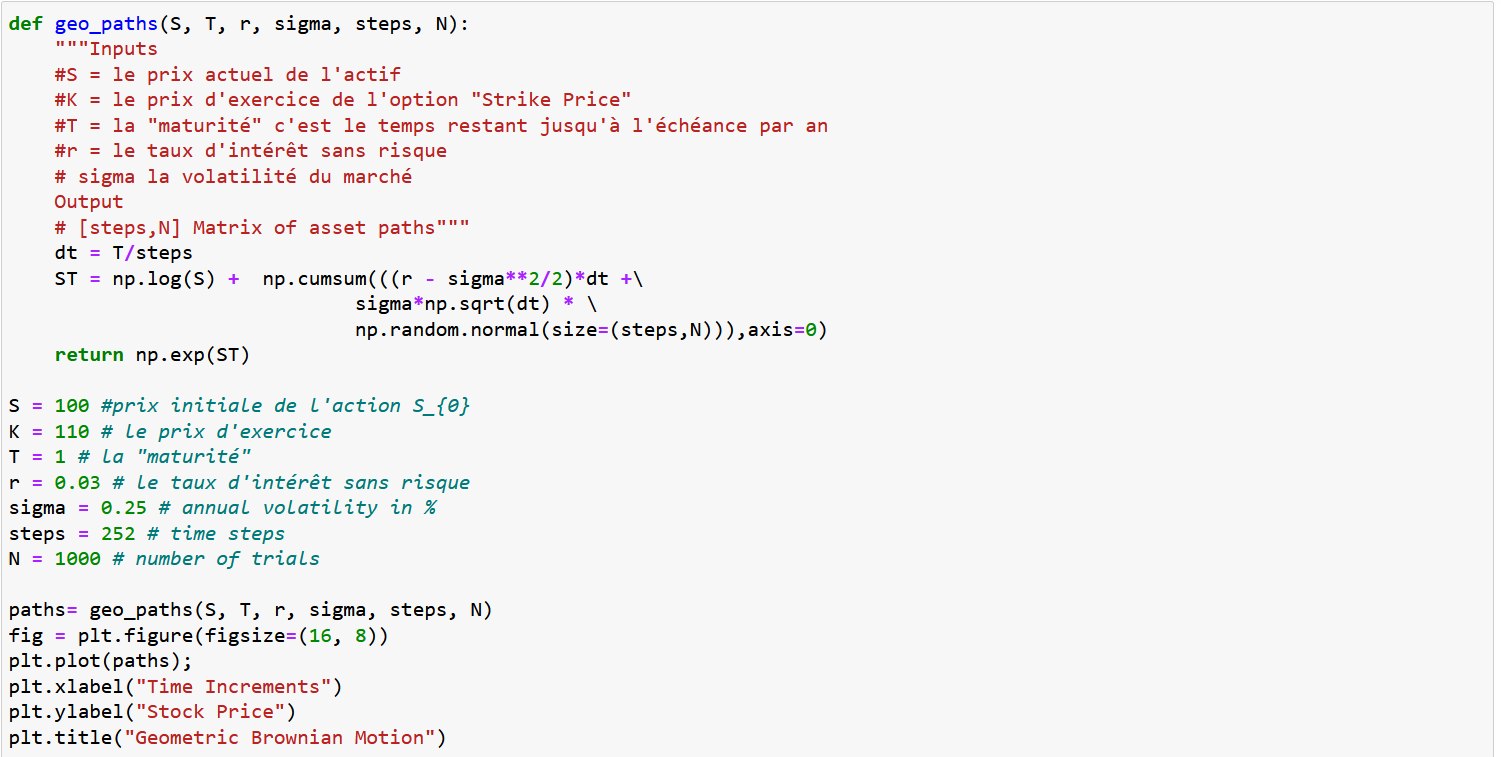
\includegraphics[scale=0.7]{Meth_sim}
  \caption{Méthode pour générer 1000 simulations}
  \label{fig:mon_image}
\end{figure}
\begin{figure}[h]
  \centering
  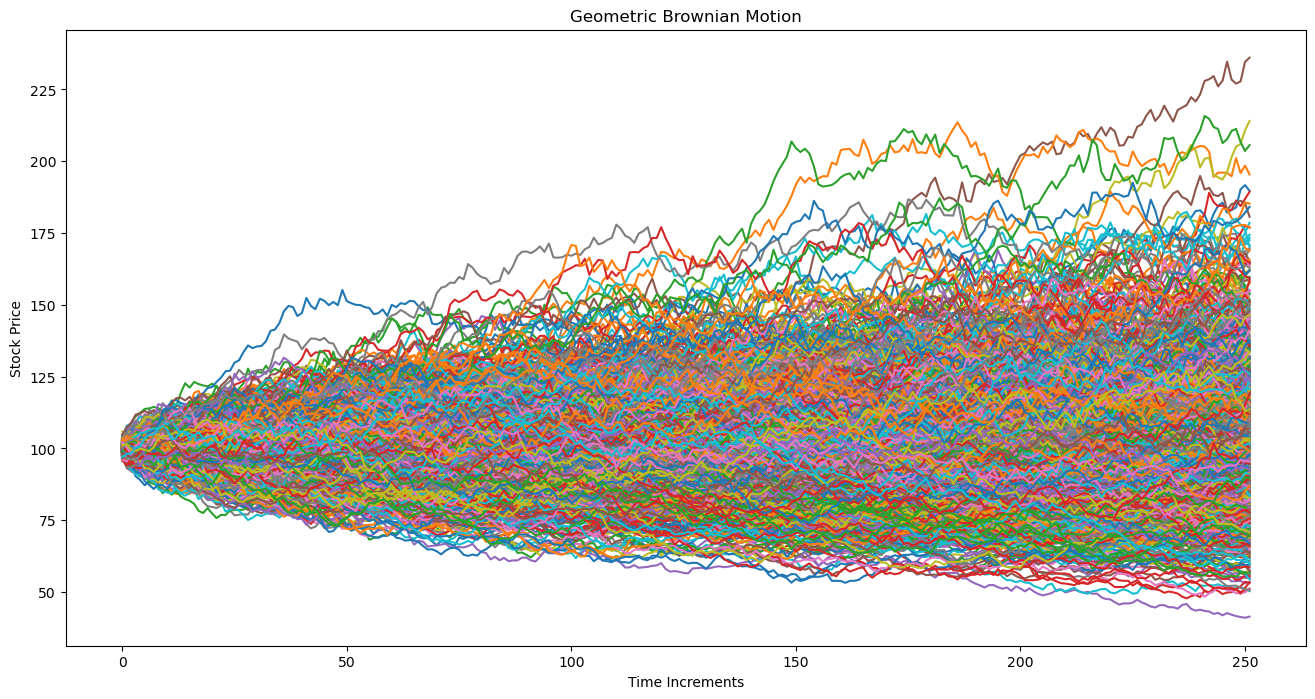
\includegraphics[scale=0.55]{res_sim}
  \caption{Affichage des simulations}
  \label{fig:mon_image}
\end{figure}
\begin{figure}[h]
  \centering
  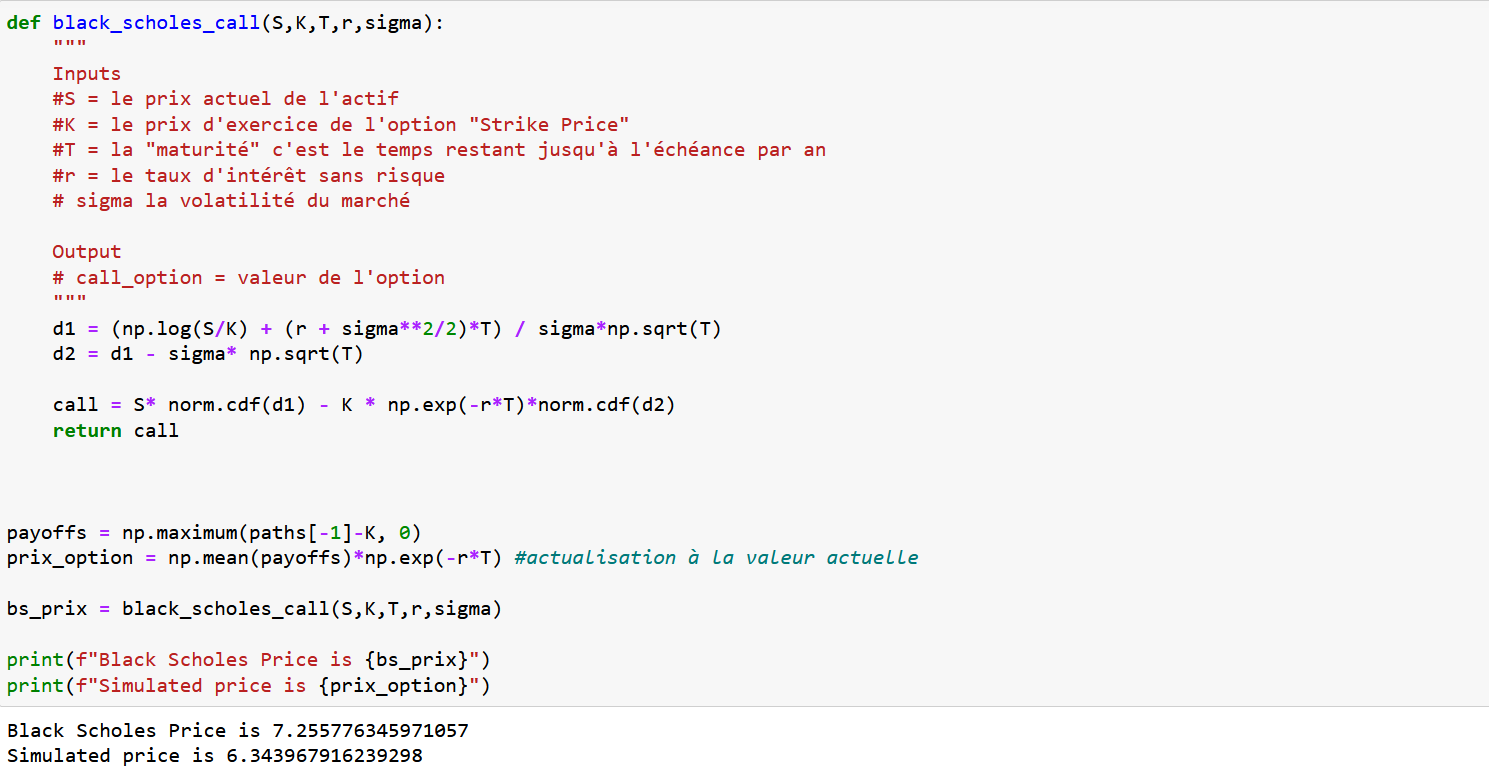
\includegraphics[scale=0.7]{sim_vs_bs}
  \caption{Comparaison entre les résultats des simulations et celles du modèle Black-Scholes}
  \label{fig:mon_image}
  La différence entre les deux prix est considérable en raison de la faible taille de l'échantillon choisi. Essayons de changer $N$ en $100000$ et de relancer le script, nous aurons:
\end{figure}

\begin{figure}[h]
  \centering
  \includegraphics[scale=0.7]{ajout_nbr_sim}
  \caption{Comparaison entre les résultats des simulations et celles du modèle Black-Scholes}
  \label{fig:mon_image}
\end{figure}
\chapter{Étude de stabilité des équations différentielles stochastiques}
Nous considérons des équations différentielles stochastiques pour lesquelles l'unicité de la trajectoire se vérifie. En utilisant le théorème de représentation de Skorokhod, nous allons établir plusieurs résultats de stabilité forte sous perturbation des conditions initiales, des coefficients, et des processus de drift. 
\section{Introduction}
Considérons l'équation différentielle stochastique suivante:
\begin{equation}\label{E50}
\left\{\begin{array}{l}
d X_{t}= b\left(t, X_{t}\right) d t + \sigma\left(t, X_{t}\right) d B_{t} \\
X_{0}=x
\end{array}\right.
\end{equation}

Où $\sigma: \R_{+} \times \R^d \longrightarrow \R^{d\times r}$ et $b: \R_{+} \times \R^d \longrightarrow \R^d$ sont des fonctions mesurables, $B$ est un mouvement Brownien définie sur un espace  de probabilité $(\Omega, \mathcal{F}, \pr)$ avec une filtration $\mathcal{F}_{t}$ satisfaisant les conditions usuelles. Dans toute la suite on va supposer que l'équation (\ref{E50}) admet une unique solution forte $X_{t}(x)$ pour toute valeur initial  $x \in \R^d$. Il est bien connu que si les coefficients sont Lipschitzienne, l'équation (\ref{E50}) a une solution unique $X_{t}(x)$, qui est continue par rapport à la condition initiale et aux coefficients. De plus, la solution peut être construite au moyen de divers schémas numériques.

Notre objectif dans ce chapitre est d'étudier les propriétés de stabilités de la solution de l'équation (\ref{E50}) sous l'hypothèse de l'unicité de la trajectoire et des conditions minimales sur les coefficients $b$ et $\sigma$ qui   assure l'existence d'une solution faible, et c'est la continuité de $b, \sigma$ par rapport aux variables d'état. Selon le théorème de Yamada-Watanabe, l'existence d'une solution faible et l'unicité de la trajectoire impliquent l'existence d'une solution forte unique.
\section{Variation de la solution par rapport aux conditions initiales}
Dans cette section nous allons étudier la variation de la solution par rapport aux conditions initiales. Nous utiliserons le théorème de sélection de Skorokhod.
\begin{theorem}[Skorokhod \cite{Ikeda}  page 9] 
Soit $(S, \rho)$ un espace métrique séparable, $\pr_{n}, n=1,2, \ldots$ et $\pr$ soient des mesures de probabilités sur $(S, \mathcal{B}(S))$ tel que $\pr_{n} \underset{n \rightarrow+\infty}{\longrightarrow}$ $\pr$. alors, dans un espace de probabilité $(\widehat{\Omega}, \widehat{\mathcal{F}}, \widehat{\pr})$, on peut construire des variables aléatoires à valeurs dans $S$, $X_{n}, n=1,2, \ldots$, et $X$ tel que:
\begin{itemize}
\item[i)] $\pr_{n}=\widehat{\pr}_{X_{n}}, n=1,2, \ldots$, et $\pr =\widehat{\pr}_{X}$.

\item[ii)] $X_{n}$ converge vers $X, \widehat{\pr}$ presque surement.

\end{itemize}
\end{theorem} 

\begin{lemma}[\cite{Ikeda} page 18] Soit $\left(X_{n}(t)\right), n=1,2, \ldots$, une suite de processus continues satisfaisant les conditions suivantes:
\begin{itemize}
\item[i)] ils existent des constantes positives $M$ et $\gamma$ tel que $\E\left[\left|X_{n}(0)\right|^{\gamma}\right] \leq M$ pour tout $n=1,2, \ldots \ldots$

\item[ii)] ils existent des constantes positives $\alpha, \beta, M_{k}, k=1,2, \ldots$, tel que: $\E\left[\left|X_{n}(t)-X_{n}(s)\right|^{\alpha}\right] \leq M_{k}|t-s|^{1+\beta}$ pour tout $n$ et $t, s \in[0, k],(k=1,2, \ldots)$.
\end{itemize}


Alors ils existent une sous suite $\left(n_{k}\right)$, un espace de probabilité  $(\widehat{\Omega}, \widehat{\mathcal{F}}, \widehat{\pr})$ et des  processus continus $\widehat{X}_{n_{k}}, k=1,2, \ldots$, et $\widehat{X}$ définie sur cet espace tel que:


\begin{enumerate}
  \item les lois de $\widehat{X}_{n_{k}}$ et de $X_{n_{k}}$ coincident.

  \item $\widehat{X}_{n_{k}}(t)$ converge vers $\widehat{X}(t)$ uniformément sur tout intervalle de temps finies $\widehat{\pr}$ presque surement.

\end{enumerate}
\end{lemma}\label{lem5}
\begin{definition}[\cite{Ouknine}]
On dit que l'équation  (\ref{E50}) satisfait l'unicité de la trajectoire si lorsque\\
 $\left(X, B,(\Omega, \mathcal{F}, \pr), \mathcal{F}_{t}\right)$ et $\left(X^{\prime}, B,(\Omega, \mathcal{F}, \pr), \mathcal{F}_{t}^{\prime}\right)$ sont des solutions faibles de l'équation (\ref{E50}) avec un espace de probabilité et un Brownien $B$ commun (possiblement relative à des filtrations différentes) tel que $\pr\left[X_{0}=X_{0}^{\prime}\right]=1$, alors $X$ et $X^{\prime}$ sont indistinguables.
\end{definition}
Dans la théorie des équations différentielles ordinaires à coefficients continus, l'unicité des solutions est suffisante pour que la solution dépend continuellement de la condition initiale. Le théorème suivant donne l'analogue du résultat ci-dessus dans le cas stochastique.
Tout d'abord nous allons citer deux inégalité qui vont nous servir dans les démonstrations de certains résultats
\begin{proposition} [Estimations importantes]\label{prop2}
Soit $X_t$ une solution de l'équation (\ref{E50}) alors $X_t$ satisfait pour tout $p>1$ et tout $T\in \R_{+}$
\begin{enumerate}
\item $\E\left[ \sup_{t\leq T} \lvert X_t \rvert^{2p} \right]<+\infty$
\item $\E\left[ \lvert X_t -X_s \rvert^{2p}\right] \leq K (t-s)^p $ 
\end{enumerate}
\end{proposition}
\begin{proof}
\textit{1)} On a \begin{align*}
\E\left[  \lvert X_t \rvert^{2p} \right] &= \E \left[ \lvert x + \int_0 ^t b(s,X_s ) ds + \int_0 ^t \sigma(s, X_s) dB_s \rvert^{2p} \right]\\
&\leq C \{\lvert x\rvert^{2p} +  \E \left[ \lvert  \int_0 ^t b(s,X_s ) ds \rvert^{2p}\right]+ \E \left[\lvert \int_0 ^t \sigma(s, X_s ) dB_s \rvert ^{2p}\right]\}\\
&\leq C \{\lvert x\rvert^{2p} +  \E \left[ \lvert  \int_0 ^t b(s,X_s) ds \rvert^{2p}\right]+ \E \left[\sup_{t\leq T}\lvert \int_0 ^t \sigma(s, X_s) dB_s \rvert ^{2p}\right]\}\\
&\leq C \{\lvert x\rvert^{2p} +  \E \left[ \lvert  \int_0 ^t b(s,X_s) ds \rvert^{2p}\right]+C_1 \E \left[ \int_0 ^T \lvert \sigma(s, X_s)\rvert^2 ds  \right]^{p}\} \text{ "BDG" }\\
&\leq C \{\lvert x\rvert^{2p} +  \E \left[   \int_0 ^t \lvert b(s,X_s) \rvert^{2p} ds \right]+C_1 T^{p-1} \E \left[ \int_0 ^T \lvert \sigma(s, X_s)\rvert^{2p} ds  \right]\} \text{ "Jensen" }\\
&\leq C \{\lvert x\rvert^{2p} +  C_2\E \left[ \lvert  \int_0 ^T (b^{2p} + \sigma^{2p}) (s,X_s) ds \rvert\right]\}\\
&\leq C \{\lvert x\rvert^{2p} +  C_3\E \left[   \int_0 ^T (1+\lvert X_s\rvert^{2p})  ds \right]\}\\
\text{Donc en passant au sup}\\
 \E\left[   \sup_{t \leq T}\lvert X_t \rvert^{2p} \right] &\leq C \{\lvert x\rvert^{2p} +  C_3T + C_3  \int_0 ^T  \E\left[   \sup_{s \leq T}\lvert X_s\rvert^{2p}\right] ds \}\\
 &\leq C_T + C_3  \int_0 ^T \E\left[   \sup_{s \leq T}\lvert X_s\rvert^{2p}\right]  ds\\
 &\leq C_T   e^{C_3T} \text{ "Lemme de Gronwal" } \\
 &< +\infty
\end{align*}
\textit{2)} \begin{align*}
\E \left[ \lvert X_t  - X_s  \rvert ^{2p}\right] &= \E \left[\lvert \int_s ^t b(u,X_u ) du + \int_s ^t \sigma(u, X_u) dB_u \rvert \right]^{2p}\\
&\leq K_1 \{\E \left[\lvert \int_s ^t b(u, X_u )du \rvert\right]^{2p} +\E\left[ \lvert \int_s ^t \sigma(u,X_u )dB_u \rvert\right]^{2p}\}\\
&\leq K_1 \{\E \left[ \int_s ^t \lvert b(u, X_u ) \rvert^2 du  \right]^{p} + \E\left[ \sup_{r \leq t}\lvert \int_s ^r \sigma(u,X_u )dB_u\rvert \right]^{2p}\} \text{ "Jensen" }\\
&\leq K_1 \{\E \left[ \int_s ^t \lvert b(u, X_u )\rvert^2 du \right]^{p} +K_2\E\left[ \int_s ^t \lvert \sigma(u,X_u )\rvert^2du \right]^p\} \text{ "BDG" }\\
&\leq K_3 \{\E \left[ \int_s ^t (1 + \lvert X_u \rvert^{2}) du \right]^{p} +\E\left[ \int_s ^t  (1 + \lvert X_u \rvert^{2}) du \right]^p\} \\
&\leq 2 K_3 \E \left[ \int_s ^t (1 + \lvert X_u \rvert^{2}) du \right]^{p}\\
&\leq 2 K_3 \left[(t-s)^p + \E \left[ \int_s ^t \lvert X_u \rvert^{2} du\right]^p \right]
\end{align*} 
Donc on a:
\begin{equation}\label{24}
\E \left[ \lvert X_t  - X_s  \rvert ^{2p}\right] \leq 2 K_3 \left[(t-s)^p + \E \left[ \int_s ^t \lvert X_u \rvert^{2} du\right]^p \right]
\end{equation}
Or en appliquant l'inégalité de Holder pour $p$ et son conjugué $\frac{p}{p-1}$ nous obtenons: \begin{align*}
\left[ \int_s ^t \lvert X_u \rvert^{2} du\right]^p &\leq \left[ \left(\int_s ^t \lvert X_u \rvert^{2p} du\right)^{\frac{1}{p}} \left(\int_s ^t du \right)^{\frac{p-1}{p}} \right]^p\\
\Rightarrow \E \left[ \int_s ^t \lvert X_u \rvert^{2} du\right]^p &\leq \E \left[ \left(\int_s ^t \lvert X_u \rvert^{2p} du\right) \left(\int_s ^t du \right)^{p-1} \right]\\
&\leq \E \left[(t-s)^{p-1} \left(\int_s ^t \lvert X_u \rvert^{2p} du\right)  \right]\\
&\leq (t-s)^{p-1} \int_s ^t \E(\lvert X_u \rvert^{2p}) du  \\
&\leq (t-s)^{p-1} \int_s ^t \E( \sup_{u \in [s,t]}\lvert X_u \rvert^{2p}) du  \\
& \leq C (t-s)^p
\end{align*}
Donc par substitution dans (\ref{24}) nous aurons:
\begin{equation}\label{25}
\E \left[ \lvert X_t  - X_s  \rvert ^{2p}\right] \leq K (t-s)^p
\end{equation}
\end{proof}
\begin{theorem}\label{thm3}
Soit $\sigma(t, x)$ et $b(t, x)$ des fonctions continus satisfaisant la condition d'accroissement lineaire: pour tout $T \geq 0$, ils existent $M$ tel que:
\begin{equation}\label{E14}
|\sigma(t, x)|+|b(t, x)| \leq M(1+|x|) \text { pour tout } t \in[0, T]
\end{equation}
Alors, si l'unicité de la trajectoire est satisfaite pour l'équation (\ref{E50}), on aura:
$$
\lim _{x \rightarrow x_{0}} \E\left[\sup _{t \leq T}\left|X_{t}(x)-X_{t}\left(x_{0}\right)\right|^{2}\right]=0, \text { pour tout } T \geq 0
$$
\end{theorem}
\begin{proof}
Supposons que la conclusion de notre théorème est fausse, alors il existe un nombre positive  $\delta$ et une suite $\left(x_{n}\right)$ convergeante vers $x$ tel que:
\begin{equation}\label{cond}
\inf _{n \in \mathbb{N}} \E\left[\sup _{t \leq T}\left|X_{t}\left(x_{n}\right)-X_{t}(x)\right|^{2}\right] \geq \delta
\end{equation}

Notons $X^{n}$ (resp. $X$ ) la solution de (\ref{E50}) correspondant à la condition initial  $x_{n}$ (resp. $x$ ).

On peut montrer que la suite $\left(X^{n}, X, B\right)$ satisfait les conditions i) et ii) du lemme \ref{lem5} avec $p>1$, grâce à la proposition \ref{prop2}.
Alors il existe un espace de probabilité $(\widehat{\Omega}, \widehat{\mathcal{F}}, \widehat{\pr})$ et une suite $\left(\widehat{X}_{t}^{n}, \widehat{Y}_{t}^{n}, \widehat{B}_{t}^{n}\right)$ de processus stochastiques  définie sur cet espace tel que:
\begin{itemize}
\item[$\alpha$)]les lois de $\left(X^{n}, X, B\right)$ et $\left(\widehat{X}^{n}, \widehat{Y}^{n}, \widehat{B}^{n}\right)$ coïncident pour tout $n \in \N$.

\item[$\beta$)]il existe une sous-suite $\left(\widehat{X}^{n_{k}}, \widehat{Y}^{n_{k}}, \widehat{B}^{n_{k}}\right)$ convergeant vers $(\widehat{X}, \widehat{Y}, \widehat{B})$ uniformément sur tout intervalle de temps finie $\widehat{\pr}$-p.s.
\end{itemize}


On note par $\widehat{\mathcal{F}}_{t}^{n}=\sigma\left(\widehat{X}_{s}^{n}, \widehat{Y}_{s}^{n}, \widehat{B}_{s}^{n} ; s \leq t\right)$ et $\widehat{\mathcal{F}}_{t}=\sigma\left(\widehat{X}_{s}, \widehat{Y}_{s}, \widehat{B}_{s} ; s \leq t\right)$, alors $\left(\widehat{B}_{t}^{n}, \widehat{\mathcal{F}}_{t}^{n}\right)$ et $\left(\widehat{B}_{t}, \widehat{\mathcal{F}}_{t}\right)$ sont des mouvements Browniens.

D'après $\alpha$ ) et le  fait que $X_{t}^{n}$ et $X_{t}$ satisfont (\ref{E50}) avec condition initiale $x_{n}$ et $x$, on peut démontrer que $\forall n \in \N, \forall t \geq 0$

$$
\E\left|\widehat{X}_{t}^{n}-x_{n}-\int_{0}^{t} \sigma\left(s, \widehat{X}_{s}^{n}\right) d \widehat{B}_{s}^{n}-\int_{0}^{t} b\left(s, \widehat{X}_{s}^{n}\right) d s\right|^{2}=0
$$

en d'autre termes , $\widehat{X}^{n}$ satisfait l'équation différentiel stochastique  :

$$
\widehat{X}_{t}^{n}=x_{n}+\int_{0}^{t} \sigma\left(s, \widehat{X}_{s}^{n}\right) d \widehat{B}_{s}^{n}+\int_{0}^{t} b\left(s, \widehat{X}_{s}^{n}\right) d s
$$

En écrivant des relations similaires, on obtient :

$$
\widehat{Y}_{t}^{n}=x+\int_{0}^{t} \sigma\left(s, \widehat{Y}_{s}^{n}\right) d \widehat{B}_{s}^{n}+\int_{0}^{t} b\left(s, \widehat{Y}_{s}^{n}\right) d s
$$

En utilisant maintenant la propriété $(\beta)$ et le théorème limite de Skorokhod \cite{Skoro} page 32, on obtient que:

$$
\begin{gathered}
\int_{0}^{t} \sigma\left(s, \widehat{X}_{s}^{n_{k}}\right) d \widehat{B}_{s}^{n_{k}} \underset{k \rightarrow+\infty}{\longrightarrow} \int_{0}^{t} \sigma\left(s, \widehat{X}_{s}\right) d \widehat{B}_{s} \\
\text { et } \int_{0}^{t} b\left(s, \widehat{X}_{s}^{n_{k}}\right) d s \underset{k \rightarrow+\infty}{\longrightarrow} \int_{0}^{t} b\left(s, \widehat{X}_{s}\right) d s  \text{ en probabilité }
\end{gathered}
$$
donc $\widehat{X}$ et $\widehat{Y}$ satisfont la même Équation Différentielle Stochastique sur $(\widehat{\Omega}, \widehat{\mathcal{F}}, \widehat{\pr})$ avec le même mouvement Brownien $\widehat{B}_t$ et la même condition initial $x$.\\
Donc par  l'unicité de la trajectoire nous déduisons que  $\widehat{X}_t =  \widehat{Y}_t$ $\forall t\geq 0$ $\widehat{\pr}-$ps.

Par intégrabilité uniforme on va obtenir:
\begin{align*}
\delta &\leq \liminf_{n \in \N} \widehat{\E} (\sup_{t\leq T} \lvert \widehat{X}_t(x_n) - \widehat{Y}_t (x)\rvert^2)\\
&\leq \liminf_{k \in \N} \widehat{\E} (\sup_{t\leq T} \lvert \widehat{X}_t ^{n_k} - \widehat{Y}_t ^{n_k} \rvert^2 )\\
&= \widehat{\E}(\sup_{t\leq T} \lvert \widehat{X}_t  - \widehat{Y}_t \rvert^2 )\\
\end{align*}
Ce qui contredit la condition (\ref{cond}).
\end{proof}
\section{Unicité de la trajectoire et approximations successives }
Prenons $\sigma$ et $b$ continues, vérifiant la condition de la croissance linéaire (\ref{E14}) (les mêmes conditions du théorème (\ref{thm3})). La suite des approximations associé à l'équation 
(\ref{E50}) est définie comme suite:\\ 
\begin{equation}\label{E15}
\left\{\begin{array}{l}
X_{t}^{n+1}=\int_{0}^{t} \sigma\left(s, X_{s}^{n}\right) d B_{s}+\int_{0}^{t} b\left(s, X_{s}^{n}\right) d s \\
X^{0}=x
\end{array}\right.
\end{equation}

Si nous supposons que les coefficient sont Lipschitziens alors la suite $(X^n)_{n \in \N}$, converge en moyenne quadratique, ce qui nous donne un moyenne efficace pour la construction de la solution unique de l'équation (\ref{E50}) (voir \cite{Ikeda}). 

Maintenant si on enlève la condition de Lipschitz imposé aux coefficients et imposer à l'équation (\ref{E50}) d'avoir une unique solution forte, aurons nous la convergence de la suite $(X^n)_{n \in \N}$ ? La réponse est non même dans le cas déterministe (voir \cite{Dieudonné} page 114-124).

Le but du théorème suivant est d'établir une condition nécessaire et suffisante additionnelle pour assurer la convergence des approximations successives.
\begin{theorem}\label{thm4}
Soient $\sigma$ et $b$ des fonctions continues à croissance linéaire alors sous l'hypothèse de l'unicité de la trajectoire la suite des approximations $(X^n)_{n \in \N}$, converge en moyenne quadratique si et seulement si $(X^{n+1} - X^n)_{n \in \N}$, converge vers 0.
\end{theorem}
\begin{lemma}\label{lem4}
Soient $(X^n)_{n \in \N}$ définie par (\ref{E15}) alors:
\begin{enumerate}
\item Pour tout $p>1$,  $$\sup_{n\in \N} \E\left[ \sup_{t\leq T}\left|X_{t}^{n}\right|^{2 p}\right]<+\infty$$ 
\item Pour tout $T>0$ et $p>1$, alors il existe une constante $C$ indépendante de $n$ tel que pour tout $s<t$ dans $[0, T]$, 
$$\E\left[\left|X_{t}^{n}-X_{s}^{n}\right|^{2 p}\right] \leq C|t-s|^{p}$$
\end{enumerate}
\end{lemma}
\begin{proof}
\begin{enumerate}

\item Pour tout $t>0$ et $n>1$, on a 
\begin{equation}\label{E16}
\left|X_{t}^{n}\right|^{2 p} \leq C_{1}\left[|x|^{2 p}+\left|\int_{0}^{t} b\left(s, X_{s}^{n-1}\right) d s\right|^{2 p}+\left|\int_{0}^{t} \sigma\left(s, X_{s}^{n-1}\right) d B_{s}\right|^{2 p}\right]
\end{equation}

Or on applique l'inégalité de Hölder  avec $p$ et $\frac{p}{p-1}$ comme composantes
\begin{align*}
\left|\int_{0}^{t} b\left(s, X_{s}^{n-1}\right) d s\right|^{2 p} &\leq \left[\left(\int_0 ^t ds\right)^{\frac{1}{q}}\left(\int_{0}^{t} \lvert b(s, X_{s}^{n-1}) \rvert ^p d s\right)^\frac{1}{p}\right]^{2p}\\
&\leq \left(t^{\frac{p-1}{p}}\right)^{2p}\left(\int_{0}^{t}\lvert b(s, X_{s}^{n-1})\rvert^p d s\right)^{2}\\
&\leq t^{2(p-1)} \int_{0}^{t}\left|b\left(s, X_{s}^{n-1}\right)\right|^{2 p} d s \\
\Rightarrow \E \left[ \left|\int_{0}^{t} b\left(s, X_{s}^{n-1}\right) d s\right|^{2 p} \right] &\leq t^{2(p-1)} \E\left[\int_{0}^{t}\left|b\left(s, X_{s}^{n-1}\right)\right|^{2 p} d s \right]
\end{align*}
De plus d'après l'inégalité Burkholder-Davis-Gundy
\begin{align*}
\E\left[\sup _{0 \leq t \leq T}\left|\int_{0}^{t} \sigma\left(s, X_{s}^{n-1}\right) d B_{s}\right|^{2 p}\right] &\leq C_{2} \E\left[\left(\int_{0}^{T}\left|\sigma\left(s, X_{s}^{n-1}\right)\right|^{2} d s\right)^{p}\right]\\
&\leq C_{2} \E\left[\left(\int_{0}^{T}ds \right)^{\frac{p-1}{p}} \left(\int_{0}^{T}\lvert \sigma\left(s, X_{s}^{n-1}\right)\rvert^{2 p} d s\right)^\frac{1}{p} \right]^p\\
& \leq C_{2} T^{p-1} \E \left[\int_{0}^{T} \lvert \sigma(s, X_{s}^{n-1}) \rvert^{2p} ds \right]
\end{align*}
Prenons l'espérance de (\ref{E16}) on aura 
\begin{align*}
\E\left[\sup_{t \leq T}\lvert X_{t}^{n}\rvert^{2 p}\right] &\leq C_{1}\left[|x|^{2 p}+\E\left|\int_{0}^{t} b\left(s, X_{s}^{n-1}\right) d s\right|^{2 p}+\E\left|\int_{0}^{t} \sigma\left(s, X_{s}^{n-1}\right) d B_{s}\right|^{2 p}\right]\\
\text{Par substitution}\\
&\leq C_{1}\left[|x|^{2 p}+t^{2(p-1)} \E\left(\int_{0}^{t}\left|b\left(s, X_{s}^{n-1}\right)\right|^{2 p} d s \right)+ C_{2} T^{p-1} \E \left(\int_{0}^{T} \lvert \sigma(s, X_{s}^{n-1}) \rvert^{2p} ds \right) \right]\\
& \leq C_1 \left(|x|^{2 p} + C_3 \E \left( \int_{0}^{T} (\lvert\sigma \rvert^{2p} + \lvert b \rvert^{2p})(s, X_{s}^{n-1})ds \right)\right)\\
\end{align*}
La croissance linéaire de $\sigma$ et $b$ entraine que: $(\lvert \sigma \rvert^{2p}+ \lvert b\rvert^{2p}) (t, x) \leq C_4 (1+ \lvert x \rvert^{2p})$ on remplace dans l'inégalité précédente nous obtenons:
\begin{align*}
\E\left[\sup_{t \leq T}\lvert X_t ^n \rvert^{2p} \right] &\leq C_1 \left( \lvert x \rvert^{2p} +C_3 \E \left( \int_{0}^{T} C_4(1+\lvert X_s ^{n-1} \rvert^{2p})ds \right) \right)\\
&\leq C_1 \left( \lvert x \rvert^{2p} + C_3 C_4 (T+ \int_{0}^{T} \E(\sup_{s\leq t} \lvert X_s ^{n-1} \rvert^{2p}) d t) \right)\\
&\leq C_5 (1+\lvert x \rvert^{2p}) +  C_5 \int_{0}^{T} \E(\sup_{s\leq t} \lvert X_s ^{n-1} \rvert^{2p}) d t
\end{align*}
Où les constantes $C_k$ dépend de $T$ de $p$ et non de $n$, puisque l'inégalité est vrai pour tout $n$, nous aurons par induction:
\begin{align*}
\E\left[\sup_{t\leq T}\lvert X_t ^n \rvert^{2p} \right] &\leq C_5 (1+\lvert x \rvert^{2p}) + C_5 \int_{0}^{T} \left[C_5 (1+\lvert x \rvert^{2p} ) +  C_5 \int_{0}^{T} \E(\sup_{s\leq t} \lvert X_s ^{n-2} \rvert^{2p}) d t\right]du\\
&\leq C_5 (1+\lvert x \rvert^{2p}) + C_5^2 (1 + \lvert x \rvert^{2p})T + C_5^2 \int_{0}^{T} \int_{0}^{T} \E(\sup_{s\leq t} \lvert X_s^{n-2}\rvert^{2p})dt du\\
&\leq C_5 (1+\lvert x \rvert^{2p})\left[ 1+C_5 T + \frac{(C_5 T)^2}{2!} + ... +\frac{(C_5 T)^n}{n!} \right]
\end{align*}
finalement nous allons obtenir: 
\begin{align*}
\sup _{n} \E\left[\sup _{t \leq T}\left|X_{t}^{n}\right|^{2 p}\right] &\leq C_{5}\left(1+|x|^{2 p}\right) \exp (C_5 T)\\
&< + \infty
\end{align*}
\item Pour le deuxième point en procédant de la même manière et en utilisant les résultats obtenues précédemment nous obtenons pour $s<t$ dans $[0, T]$, 
\begin{align*}
\E\left[\left|X_{t}^{n}-X_{s}^{n}\right|^{2 p}\right] &\leq \E \left[\int_s ^t b(u,X_u ^n) du + \int_s ^t \sigma(u, X_u ^n) dB_u \right]^{2p}\\
&\leq K_1 \E\left[(t-s)^{2(p-1)} \int_s ^t \lvert b(u,X_u ^n) \rvert^{2p} du + K_2 (t-s)^{p-1} \int_s ^t \sigma(u, X_u ^n) du \right]\\
&\leq K_1 \E\left[K_3(t-s)^{p-1} \int_s ^t \lvert b(u,X_u ^n) \rvert^{2p} du + K_2 (t-s)^{p-1} \int_s ^t \sigma(u, X_u ^n) du \right]\\
&\leq K_4 (t-s)^{p-1}  \int_{s}^{t} \E \left[1+ \sup_{v \leq u} \lvert X_v ^{n-1}\rvert^{2p} \right] du\\
&\leq K_{5}(t-s)^{p-1} \int_{s}^{t} (1 + \E\left[\sup _{v \leq u}\left|X_{v}^{n-1}\right|^{2 p}\right] d u)\\
&\leq K_6 (t-s)^{p}
\end{align*}
Où $K_6$ dépend de $x$, $p$ et de $T$.
\end{enumerate}

\end{proof}
\begin{proof}[\textbf{Preuve du théorème \ref{thm4}}]
Supposons que $(X^{n+1}-X^{n}, n \in \N)$ converge vers 0 et qu'il existe un $\delta>0$ tel que:

$$
\inf _{n} \E\left[\max _{0 \leq t \leq T}\left|X_{t}^{n}-X_{t}\right|^{2}\right] \geq \delta
$$

d'après le lemme (\ref{lem4}), la famille $\left(X^{n}, X^{n+1}, X, B\right)$, satisfait les  conditions du lemme (\ref{lem5}). donc par le théorème de Skorokhod, il existe un espace de probabilité  $(\widehat{\Omega}, \widehat{\mathcal{F}}, \widehat{\pr})$ et une suite de processus $\left(\widehat{X}^{n}, \widehat{Z}^{n}, \widehat{Y}^{n}, \widehat{B}^{n}\right)$ avec les  propriétés suivantes:
\begin{itemize}
\item[i)] les lois de $\left(\widehat{X}^{n}, \widehat{Z}^{n}, \widehat{Y}^{n}, \widehat{B}^{n}\right)$ et $\left(X^{n}, X^{n+1}, X, B\right)$ coïncident pour tout $n \in N$
\item[ii)] ils existent une sous-suite $\left\{n_{k}\right\}$ tel que $\left(\widehat{X}^{n_{k}}, \widehat{Z}^{n_{k}}, \widehat{Y}^{n_{k}}, \widehat{B}^{n_{k}}\right)$ converge vers $(\widehat{X}, \widehat{Z}, \widehat{Y}, \widehat{B})$ uniformément sur tout intervalle de temps finie $\widehat{\pr}$-p.s.
\end{itemize} 

Or on sait que $(X^{n+1}-X^{n}, n\in \N)$ converge vers 0, on peut montrer facilement que $\widehat{X}=\widehat{Z}, \widehat{\pr}$-ps.
On procède de la même manière vu précédemment
$$
\begin{aligned}
 \widehat{Z}^{n_{k}}=x+\int_{0}^{t} b\left(s, \widehat{X}^{n_{k}}\right) d s + \int_{0}^{t} \sigma\left(s, \widehat{X}^{n_{k}}\right) d \widehat{B}_{s}^{n_{k}} \\
 \widehat{Y}^{n_{k}}=x +\int_{0}^{t} b\left(s, \widehat{Y}_{s}^{n_{k}}\right) d s + \int_{0}^{t} \sigma\left(s, \widehat{Y}_{s}^{n_{k}}\right) d \widehat{B}_{s}^{n_{k}}
\end{aligned}
$$

passaons à la limite quand $k$ tend vers $+\infty$ nous aurons

$$
\begin{aligned}
& \widehat{X}_{t}=x+\int_{0}^{t} b\left(s, \widehat{X}_{s}\right) d s +\int_{0}^{t} \sigma\left(s, \widehat{X}_{s}\right) d \widehat{B}_{s}\\
& \widehat{Y}_{t}=x+\int_{0}^{t} b\left(s, \widehat{Y}_{s}\right) d s +\int_{0}^{t} \sigma\left(s, \widehat{Y}_{s}\right) d \widehat{B}_{s}
\end{aligned}
$$

En d'autre terme, $\widehat{X}$ et $\widehat{Y}$ sont des solutions de l'équation (\ref{E50}). Alors l'hypothèse de l'unicité de la trajectoire $\widehat{X}=\widehat{Y}, \widehat{P}$-p.s.
En utilisant l'intégrablité uniforme:
$$
\begin{aligned}
\delta & \leq \liminf _{k} \E\left[\max _{0 \leq t \leq T}\left|X_{t}^{n_{k}}-X_{t}\right|^{2}\right]=\liminf _{k} \widehat{\E}\left[\max _{0 \leq t \leq T}\left|\widehat{X}_{t}^{n_{k}}-\widehat{Y}_{t}^{n_{k}}\right|^{2}\right] \\
& =\widehat{\E}\left[\max _{0 \leq t \leq T}\left|\widehat{X}_{t}-\widehat{Y_{t}}\right|^{2}\right]
\end{aligned}
$$
D'où la contradiction.
\end{proof}
\section{Discontinuité du processus drift}
Dans cette section on enlève l'hypothèse de continuité du processus drift $b$.
Supposons que $b$ borélienne, bornée et non continue et on pose $\sigma =1$.
Nous allons tout d'abord citer deux lemmes qui vont  nous servir dans la démonstration du théorème
\begin{lemma}[\cite{MERKER} page 20] 
Soit $f \in L^p$, $\varphi \in C_c^{\infty}(\R^d)$ tel que $\int_{\R^d} \varphi d \mu =1 $ et $\varphi \geq 0$. posons pour $\delta > 0$, $$\varphi_{\delta} (x) = \frac{1}{\delta^d} \varphi(\frac{x}{\delta})$$
Alors $f*\varphi_{\delta} \rightarrow f$ dans $L^p$ lorsque $\delta \rightarrow 0$, où $*$ désigne le produit de convolution sur $\R^d$.

\end{lemma}\label{lem6}
\begin{lemma}[Inégalité de Krylov \cite{Cavallazzi} page 11 ] 
Si $X$ est solution de l'équation (\ref{E50}), alors pour toute fonction positive  $g : [0, T] \times \R^d \longrightarrow \R^d _{+} $ progressivement mesurable nous avons:
\begin{align*}
\E \left[\int_0 ^T g(t,X_t)dt \right] & \leq M \left( \int_0^T \int_{\R^d} g^{d+1}(t,x)dx dt \right)^{\frac{1}{d+1}} \\
&\leq M \parallel g \parallel_{L^{d+1} ([0, T]\times \R^d)}
\end{align*} 
\end{lemma}\label{lem7}

\begin{theorem}
Supposons que $b$ borélienne, bornée et non continue et on pose $\sigma =1$. On suppose de plus que l'unicité de la trajectoire est satisfaite. Alors la conclusion du théorème \ref{thm3} est satisfaite.
\end{theorem} 
\begin{proof}
La preuve se déroule comme dans la preuve du théorème \ref{thm3} sauf quelques changements.
Par l'absurde on suppose que:
\begin{equation}
\inf _{n \in \mathbb{N}} \E\left[\sup _{t \leq T}\left|X_{t}\left(x_{n}\right)-X_{t}(x)\right|^{2}\right] \geq \delta
\end{equation}
$(X^n, X, B)$ satisfont $i)$ et $ii)$ du lemme \ref{lem5}  grâce à la proposition \ref{prop2}.
de même pour $X$ et $B$, alors il existe un espace de probabilité $(\widehat{\Omega}, \widehat{\mathcal{F}}, \widehat{P})$, et une suite  $\left(\widehat{X}^{n}, \widehat{Y}^{n}, \widehat{B}^{n}\right)$ de processus définie sur cette espace tel que:
\begin{enumerate}
\item Les lois de $(X^n, X, B)$ et $(\widehat{X}^n, \widehat{Y}^n, \widehat{B}^n)$ coïncident  $\forall n \in \N $
\item Il existe une suite $(\widehat{X}^{n_k}, \widehat{Y}^{n_k}, \widehat{B}^{n_k})$ convergeant vers $(\widehat{X}, \widehat{Y}, \widehat{B})$, uniformément sur tout intervalle de temps finie $\widehat{\pr}-ps$. 
\end{enumerate}
d'après le premier point et le fait que $X_t$ et $X_t ^n$ satisfont (\ref{E50}) avec condition initiale $x_n$ et $x$,
$$
\E\left|\widehat{X}_{t}^{n}-x_{n} - \int_{0}^{t} b\left(s, \widehat{X}_{s}^{n}\right) d s -\int_{0}^{t} d \widehat{B}_{s}^{n} \right|^{2}=0
$$
en d'autre termes $\widehat{X}^n$, satisfait l'équation (\ref{E50}) de même pour $\widehat{Y}_t ^n$.
La difficulté réside dans 
$$
\begin{gathered}
\int_{0}^{t} b\left(s, \widehat{X}_{s}^{n_{k}}\right) d s \underset{k \rightarrow+\infty}{\longrightarrow} \int_{0}^{t} b\left(s, \widehat{X}_{s}\right) d s \text{ en probabilité }
\end{gathered}
$$
Soit $\varepsilon > 0$, on a: 
$$\lim_{k \rightarrow +\infty} \pr\left( \left| \int_0 ^t b(s, \widehat{X}_{s}^{n_{k}}) ds - \int_0 ^t b(s, \widehat{X}_{s}) ds \right| > \varepsilon \right)= \lim_{k \rightarrow +\infty} \pr\left( \left| \int_0 ^t (b(s, \widehat{X}_{s}^{n_{k}}) -  b(s, \widehat{X}_{s})) ds \right| > \varepsilon \right) $$ 
Définissons d'abord $$b^{\delta} (t,x) = \delta^{-d} \varphi(\frac{x}{\delta})*b(t,x) $$ où $\varphi$ et $C^{\infty}$ à support dans la boule unité et $\int \varphi(x)dx =1$.
L'inégalité de Tchebychev nous donne:
\begin{align*}
\pr\left( \left| \int_0 ^t (b(s, \widehat{X}_{s}^{n_{k}})- b(s, \widehat{X}_{s})) ds \right| > \varepsilon\right) &\leq \frac{1}{\varepsilon^2} \E \left[ \left| \int_0 ^t (b(s, \widehat{X}_{s}^{n_{k}})- b(s, \widehat{X}_{s}))ds \right|^2 \right]\\
&\leq \frac{1}{\varepsilon^2} \E \left[ \left| \int_0 ^t (b(s, \widehat{X}_{s}^{n_{k}})-b^{\delta}(s, \widehat{X}_{s}^{n_{k}})) \right. \right. \\
&\phantom{\leq \frac{1}{\varepsilon^2} \E \left[ \right]} + \left. \left. (b^{\delta}(s, \widehat{X}_{s} ^{n_{k}}) - b^{\delta}(s, \widehat{X}_{s})) \right. \right. \\
&\phantom{\leq \frac{1}{\varepsilon^2} \E \left[ \right]} + \left. \left. (b^{\delta}(s, \widehat{X}_{s}) - b(s, \widehat{X}_{s})) \right|^2  ds \right] \\
& \leq \frac{3}{\varepsilon^2} \lbrace \E \left[ \int_0 ^t \rvert b(s, \widehat{X}_{s}^{n_{k}})-b^{\delta}(s, \widehat{X}_{s}^{n_{k}}) \rvert^2 ds \right]\\
& + \E \left[ \int_0 ^t \lvert b^{\delta}(s, \widehat{X}_{s} ^{n_{k}}) - b^{\delta}(s, \widehat{X}_{s}) \rvert^2 ds \right]\\
& + \E \left[ \int_0 ^t \lvert b^{\delta}(s, \widehat{X}_{s}) - b(s, \widehat{X}_{s}) \rvert^2 ds \right]\rbrace\\
&\leq \frac{3}{\varepsilon^2} ( I_1 + I_2 + I_3)
\end{align*}
Comme $\widehat{X}_{s} ^{n_{k}}$ converge uniformément sur tout intervalle de temps fini $\widehat{\pr}$-ps vers $\widehat{X}_{s} $ quand $k \longrightarrow + \infty$, et $b^{\delta}$ est continue on aura $I_2 \longrightarrow 0 $, quand $k \longrightarrow +\infty$.\\
Or pour $$I_1 = \E \left( \int_0 ^t \rvert b(s, \widehat{X}_{s}^{n_{k}})-b^{\delta}(s, \widehat{X}_{s}^{n_{k}}) \rvert^2 ds \right)$$ 
On considère une fonction de troncature $\theta : \R^d \longrightarrow \R_+$ tel que 
$$
\theta(x) = \left\{
    \begin{array}{ll}
        0 & \mbox{si } \lvert x \rvert > 1\\
        1 & \mbox{si }  \lvert x \rvert \leq 1
    \end{array}
\right.
$$
Nous obtenons:
\begin{align*}
I_1 = &\E \left( \int_0 ^t \theta(\widehat{X}_{s}^{n_{k}}/R)(\rvert b(s, \widehat{X}_{s}^{n_{k}})-b^{\delta}(s, \widehat{X}_{s}^{n_{k}}) \rvert^2 ds \right)\\ 
&+ \E \left( \int_0 ^t (1-\theta(\widehat{X}_{s}^{n_{k}}/R))(\rvert b(s, \widehat{X}_{s}^{n_{k}})-b^{\delta}(s, \widehat{X}_{s}^{n_{k}}) \rvert^2 ds \right)\\
& \leq N \parallel b^{\delta}- b \parallel_{L^{d+1} ([0, T]\times B(0, R))} +2C \E \left( \int_0 ^t (1-\theta(\widehat{X}_{s}^{n_{k}}/R))\right)
\end{align*}
Où $N$ ne dépend pas ni de $\delta$ ni de $k$. Or:

$$
1- \theta(\widehat{X}_{s}^{n_{k}}/R) = \left\{
    \begin{array}{ll}
        0 & \mbox{si } \lvert \widehat{X}_{s}^{n_{k}} \rvert/R \leq 1 \\
        1 & \mbox{sinon.}
    \end{array}
    = \mathbf{1}_{\{\lvert \widehat{X}_{s}^{n_{k}} \rvert > R\} }
\right.
$$
donc 
\begin{align*}
\E \left( \int_0 ^t (1-\theta(\widehat{X}_{s}^{n_{k}}/R))ds \right) &= \E \left( \int_0^t \mathbf{1}_{\{\lvert \widehat{X}_{s}^{n_{k}}\rvert  > R\} } ds \right)\\
& = \int_0^t \E \left(  \mathbf{1}_{\{\lvert \widehat{X}_{s}^{n_{k}}\rvert  > R\} } \right) ds \\
& = \int_0^t \pr(\lvert \widehat{X}_{s}^{n_{k}}\rvert > R)ds\\
&\leq \int_0^t \pr (\sup_{s\leq t}\lvert \widehat{X}_{s}^{n_{k}}\rvert > R)ds \\
&\leq \int_0^t \sup_{k \geq 1} \pr(\sup_{s\leq t}\lvert \widehat{X}_{s}^{n_{k}}\rvert > R)ds\\ 
&\leq T \sup_{k \geq 1} \pr(\sup_{s\leq t}\lvert \widehat{X}_{s}^{n_{k}}\rvert > R) 
\end{align*}
Or on sait que $\sup_{k\geq 1} \E(\sup_{s\leq t}\lvert \widehat{X}_{s}^{n_{k}}\rvert^p > R) < +\infty $ pour tout $p>1$ donc $$\lim_{R\rightarrow +\infty} \sup_{k \geq 1} \pr(\sup_{s\leq t}\lvert \widehat{X}_{s}^{n_{k}}\rvert > R)=0 $$
\end{proof}
\chapter*{Conclusion}
L'unicité de la trajectoire nous a permet dans un premier temps d'examiner la sensibilité de la solution par rapport aux variations de la  condition initiale, de quantifier l'impact des variations des conditions initiales sur le comportement du système à long terme, ensuite elle nous a assurer la convergence des approximations successives qui donne un moyen efficace pour la construction de la solution unique. Enfin, l'étude de la discontinuité du processus drift a mis en évidence les effets perturbateurs que les discontinuités peuvent avoir sur les solutions des équations différentielles stochastiques. Comprendre ces aspects est essentiel pour analyser correctement la stabilité des équations différentielles stochastiques.

Dans l'ensemble, l'étude de la stabilité des équations différentielles stochastiques sous l'hypothèse de l'unicité de trajectoire offre un cadre solide pour analyser les systèmes dynamiques soumis à des perturbations aléatoires. Ces études nous permettent de mieux appréhender les comportements complexes des processus stochastiques et d'évaluer leur stabilité à long terme. En continuant à approfondir ces recherches, nous pourrons renforcer notre compréhension des phénomènes aléatoires et améliorer nos capacités de modélisation et de prédiction dans divers domaines scientifiques et appliqués.
\begin{thebibliography}{99}
		\bibitem {Ouknine}  K. Bahlali, B. Mezerdi, Y. Ouknine: \textit{Pathwise Uniqueness and Approximation of Solutions of Stochastic Differential Equations.  } Springer-Verlag, 1998.\label{Ouknine}
		 \bibitem {Klebaner} F. C Klebaner: \textit{Introduction to Stochastic Calculus with Applications.} Imperial College Press, 2005.  \label{Klebaner}
		 \bibitem {Cavallazzi} T. Cavallazzi: \textit{Itô-Krylov’s Formula for a Flow of Measures.} HAL, 2021.\label{Cavallazzi}
		 \bibitem {Dieudonné} J. Dieudonné: \textit{Choix d’oeuvres mathématiques.}  Tome 1, Hermann Paris
(1987)\label{Dieudonné} 
		\bibitem {Eddahbi} M. Eddahbi: \textit{Introduction aux Equations Différentielles Stochastiques et Applications. } 2008.\label{Eddahbi}
		\bibitem { KHARROUBI} R. Elie, I. Kharroubi: \textit{Calcul Stochastique Appliqué à la Finance.}  \label{KHARROUBI}
	\bibitem {Le Gall.}J. F Le Gall: \textit{Mouvement Brownien, Martingales et Calcul stochastique.}  Springer-Verlag,  Heidelberg, 1991.\label{Le Gall}
	\bibitem {Gallardo}L. Gallardo: \textit{Brownian Motion and Stochastic Calculus.} Hermann, 2008. \label{Gallardo}
	\bibitem {Ikeda}  N. Ikeda, S. Watanabe: \textit{Stochastic differential equations and diffusion processes.}  North-Holland, Amsterdam (Kodansha Ltd, Tokyo ) (1981).\label{Ikeda} 
	\bibitem {Jeanblanc}M. Jeanblanc: \textit{Cours de Calcul Stochastique Master 2IF EVRY.} 2006.  \label{Jeanblanc}
	\bibitem {Karatzas} I. Karatzas, S. E. Shreve: \textit{Brownian Motion and Stochastic Calculus.} Springer-Verlag, 1991.\label{Karatzas}	  
          \bibitem {MERKER} J.Merker : \textit{ Convolution et régularisation.} Faculté des Sciences d'Orsay 2014.
          \label{MERKER}
     \bibitem {Skoro}  A.V. Skorokhod: \textit{ Studies in the theory of random processes.} Addison Wesley (1965), originally published in Kiev in (1961).\label{Skoro}
\end{thebibliography}
 
\end{document}

 


